\chapter{Konstrukce}
\label{4-algoritmus}

\section{Ovládání ESC (regulátorů otáček)}
Regulátor je ovládán přes různé komunikační protokoly. Komunikační protokoly jsou buď analogové nebo digitální. Mezi analogové protokoly patří standartní PWM signál, OneShot125, OneShot42 a MultiShot, mezi digitální patří  DSHOT300, DSHOT600 a DSHOT1200. \cite{comregul}\\
Standartní PWM signál není klasický PWM signál, kterým se například reguluje výkon žárovky. Standartní PWM signál definuje nulový výkon motoru pro pulz o délce 1ms a maximální výkon o délce 2ms. Teoretická frekvence je 500Hz, lze tedy měnit rychlost motorů 500krát za vteřinu.\\
Ostatní protokoly jsou sice rychlejší, ale nemá smysl je implementovat na platformu Arduino z důvodu malého výkonu platformy.\\ 

\begin{table}[H]
\centering
	\begin{tabular}{|l|l|l|l|}
		\hline
		\textbf{Protokol} & \textbf{Frekvece} & \textbf{Min pulz} & \textbf{Max pulz} \\ \hline
		Standart PWM      & 500 Hz            & 1000 µs            & 2000 µs            \\ \hline
		OneShot125        & 4 kHz             & 125 µs             & 250 µs             \\ \hline
		OneShot42         & 12 kHz            & 42 µs              & 84 µs              \\ \hline
		MultiShot         & 40 kHz            & 12.5 µs            & 25 µs              \\ \hline
	\end{tabular}
\caption{Analogové komunikační protokoly pro regulátory otáček}
\end{table}

\begin{table}[H]
	\centering
	\begin{tabular}{|l|l|}
		\hline
		\textbf{Protokol} & \textbf{Rychlost komunikace} \\ \hline
		DSHOT150          & 150 000 bps                  \\ \hline
		DSHOT300          & 300 000 bps                  \\ \hline
		DSHOT600          & 600 000 bps                  \\ \hline
		DSHOT1200         & 1200 000 bps                 \\ \hline
	\end{tabular}
\caption{Digitální komunikační protokoly pro regulátory otáček}
\end{table}

\textbf{PWM}\\
PWM modulace je určená pro přenos analogového signálu pomocí dvou hodnot (Low a High), přenos probíhá na digitálních pinech. Přenášená hodnota je zaimplementována do poměru High/Low. Poměr se nazývá střída a nabývá hodnot 0-100 procent. Hodnoty Low a High se zapisují v cyklu.\cite{pwmwiki}\\


%http://1oomzzme3s617r8yzr8qutjk-wpengine.netdna-ssl.com/wp-content/uploads/2017/04/Fig-1-pwm.gif
%pwm
\begin{figure}[H]
	\centering
	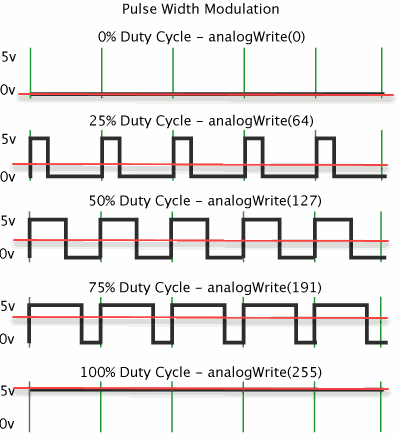
\includegraphics[width=10cm]{pictures/pwm.png}
	\caption{Ukázka PWM}
	\cite{pwm}\\
\end{figure}


\section{Kalibrace regulátorů otáček}
%https://www.youtube.com/watch?v=61bjFxJyOLU&t=52s
%blheli
Kalibrace regulátorů je nutná pro definování komunikačního protokolu a různých funkcí.\\
Pro kalibraci je potřeba kalibrovaný regulátor, propojovací dráty a Arduino Nano. V programu BLHeliSuite lze kalibrovat i s jinou platformou Arduino, bohužel kalibrace se podařila pouze s deskou typu Nano. Zapojení regulátoru se provede přes schéma na obrázku 5.2.\\
Po zapojení komponent a nastavení šablony se vybere sériový port pro komunikaci mezi počítačem a Arduinem. Přes tlačítko Read Setup se načte tovární nastavení regulátoru.\cite{blheli}\\
\begin{figure}[H]
	\centering
	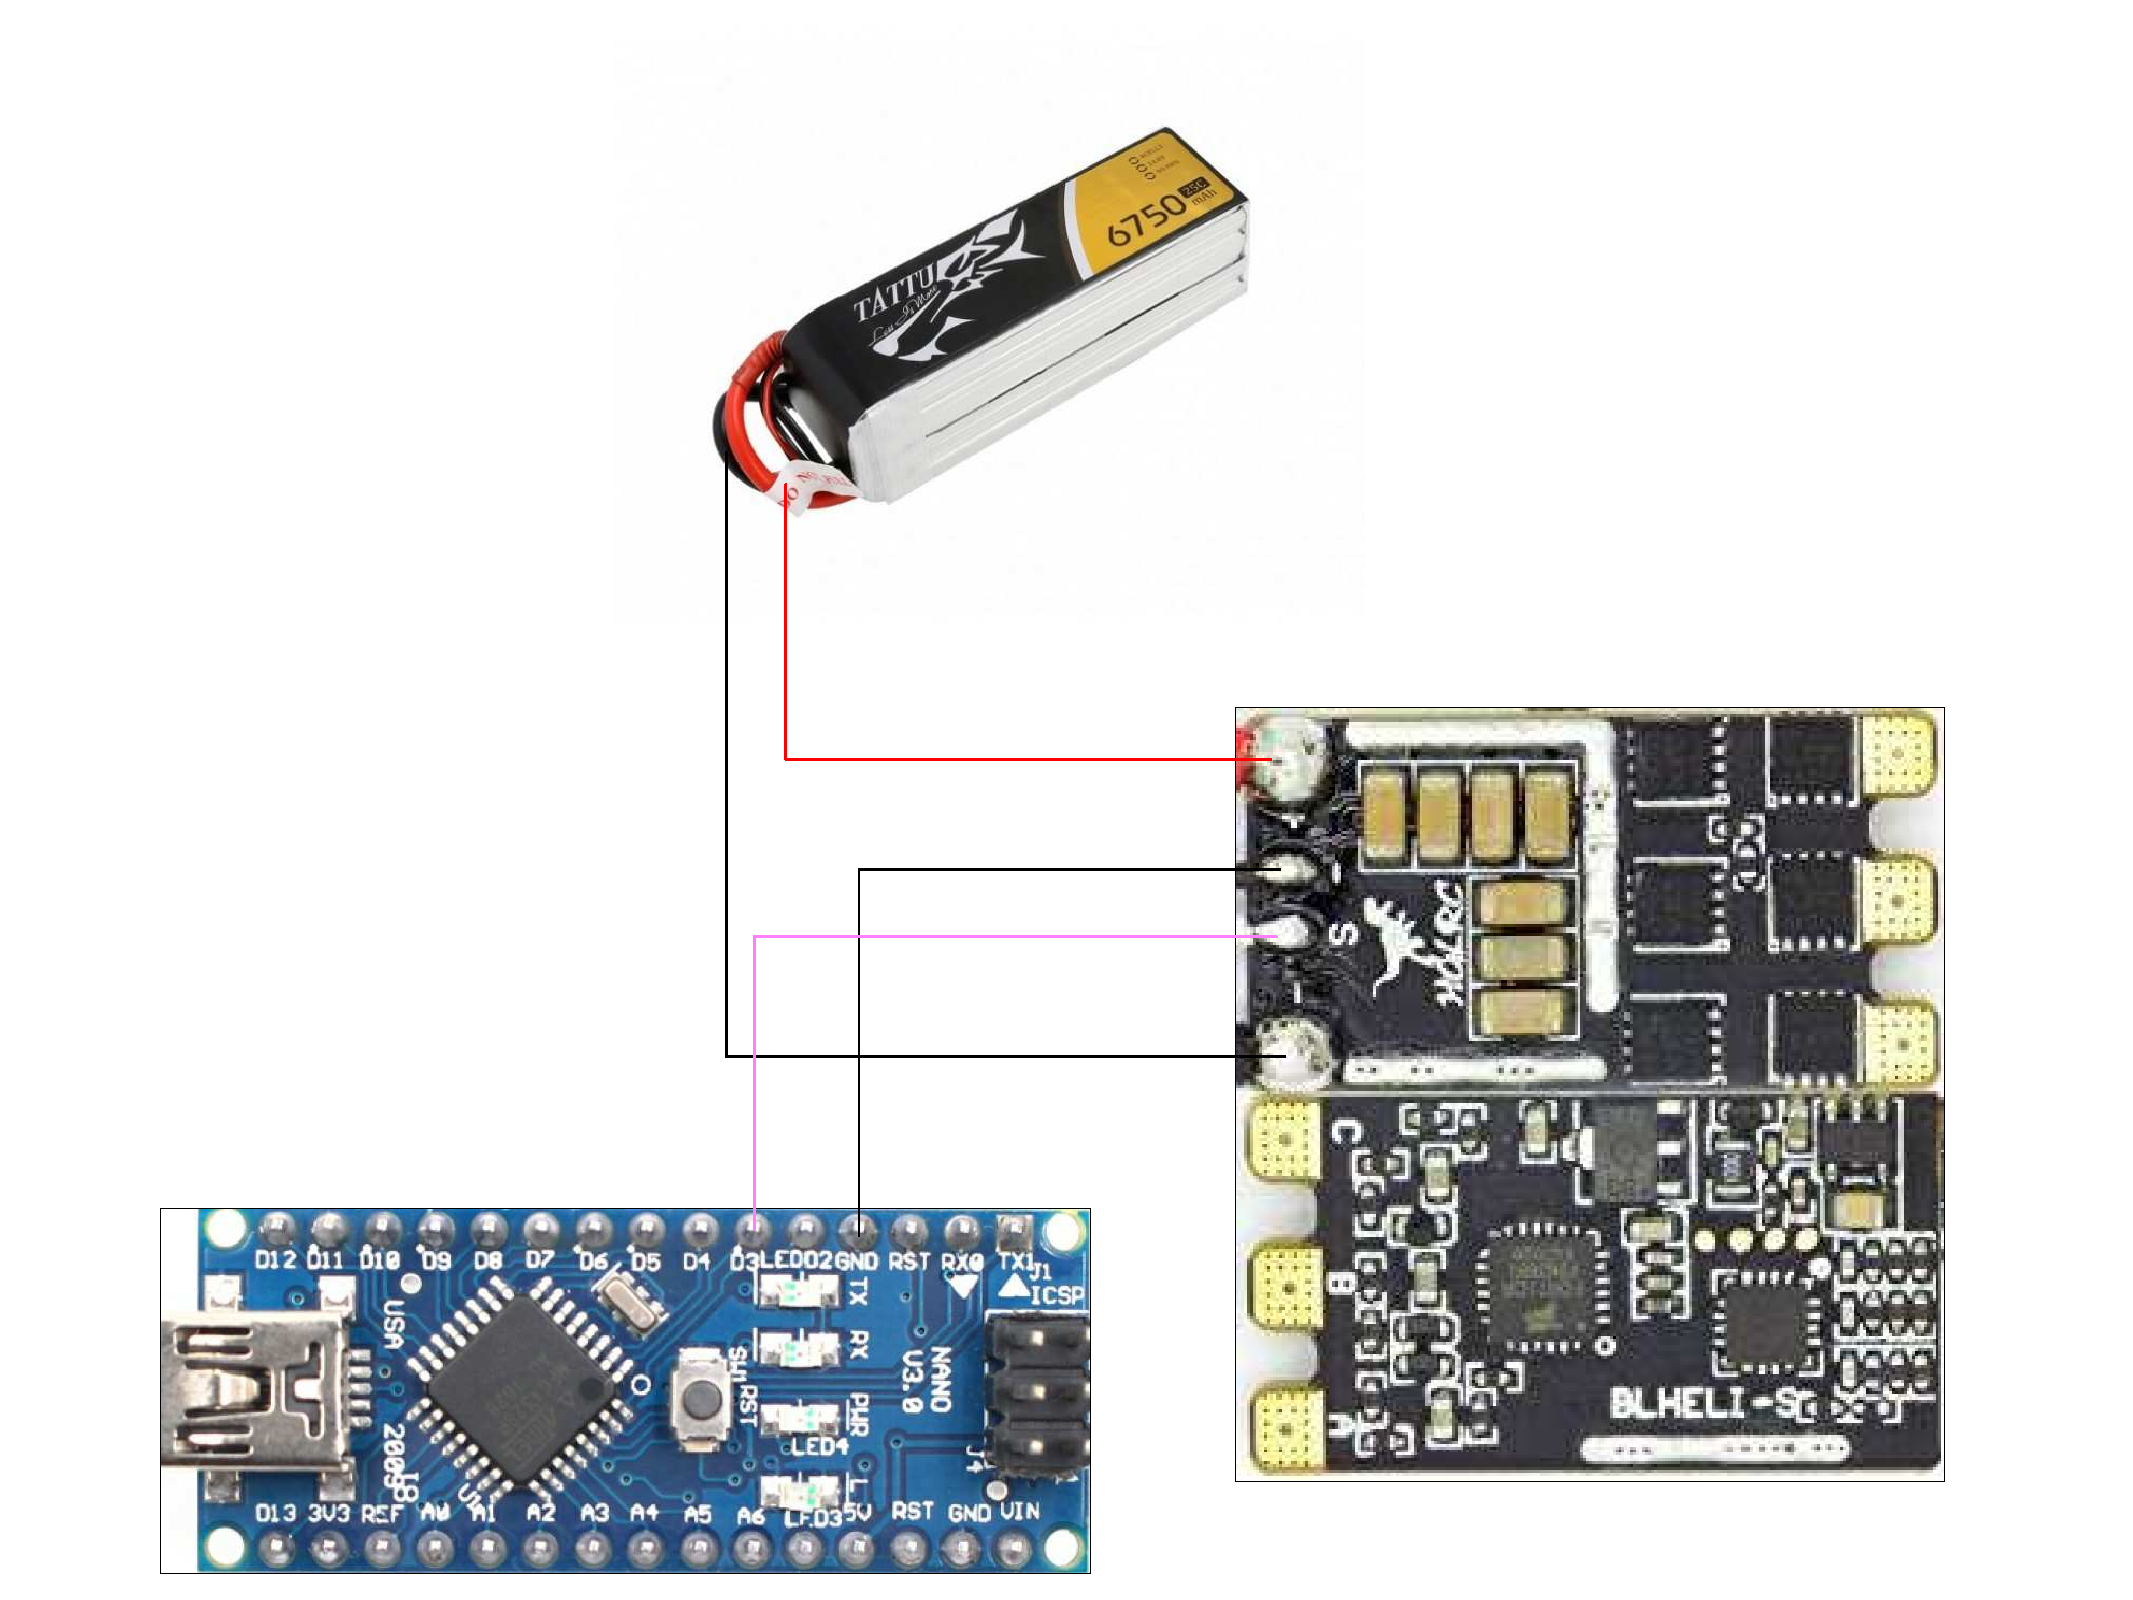
\includegraphics[width=12cm]{pictures/esc_calib.pdf}
	\caption{Schéma zapojení pro kalibraci regulátoru otáček}
\end{figure}
Nastaví se PPM Min Throttle hodnota na 1000, PPM Max Throttle na 2000 a PPM Center Throttle na 1500. Zapíše se hodnota do regulátoru. Výsledkem jsou zkalibrované vstupní hodnoty pulzu do intervalu <1000;2000>. PPM je jiný typ modulace než PWM, k ovládání regulátorů otáček stačí znát pouze PWM modulaci.\\

\begin{figure}[H]
	\centering
	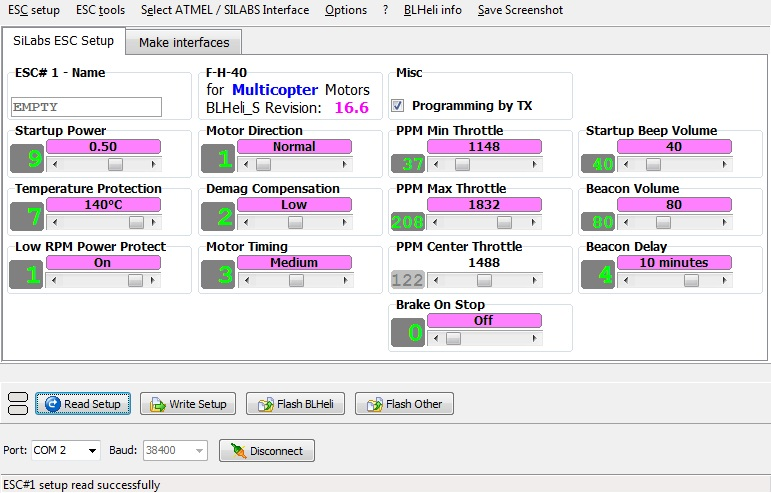
\includegraphics[width=12cm]{pictures/esc_calib5.jpg}
	\caption{Ukázka kalibrace v programu HLBeliSuite před kalibrací}
\end{figure}

\begin{figure}[H]
	\centering
	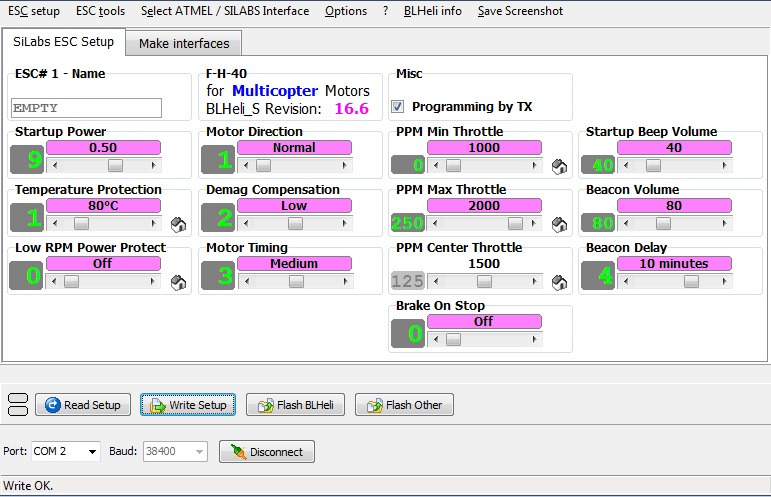
\includegraphics[width=12cm]{pictures/esc_calib6.jpg}
	\caption{Ukázka kalibrace v programu HLBeliSuite po kalibraci}
\end{figure}

\section{Filtrace dat IMU}
\textbf{Výpočet úhlů pitch a roll z dat akcelerometru.}\\
\begin{eqnarray*} 
	pitchAcc & = & atan2 (yAcc , \sqrt{xAcc^{2} + zAcc^{2}})\\
	rollAcc & = & atan2 (xAcc , \sqrt{yAcc^{2} + zAcc^{2}})\\
\end{eqnarray*} 
\textbf{Výpočet úhlů pitch a roll z dat gyroskopu}\\
Jelikož gyroskop měří úhlovou rychlost, úhly pitch a roll jsou určeny integrací z počátečního stavu. Pokud IMU jednotka nebude v počátečním stavu ve vodorovné poloze, úhly pitch a roll nebudou absolutní.\\
\begin{eqnarray*} 
	pitchGyro & = & pitchGyro + xGyro * dt\\
	rollGyro & = & rollGyro + yGyro * dt\\
	yawGyro & = & yawGyro + zGyro * dt\\
\end{eqnarray*} 
\textbf{Výpočet úhlů yaw z dat magnetometru.}\\
Při výpočtu úhlu yaw z dat magnetometru je nutné zahrnout magnetickou deklinaci, které je závislá na zeměpisných souřadnicích. \cite{declination}\\
\begin{eqnarray*} 
	yawMag & = & atan2(yMag, xMag)+ declinationMag\\
\end{eqnarray*} 

Surová data ze všech tří senzorů nejsou použitelná pro výpočet úhlů náklonu, obsahují nepřesnosti a šum, proto je potřebná filtrace.\\

%https://aip.scitation.org/doi/pdf/10.1063/1.5018520

\subsection{Komplementární filtr}
Komplementární filtr je nejjednodušší z uvedených filtrů. Využívá data z akcelerometru a gyroskopu. \\
Z dlouhodobého hlediska data z gyroskopu konvergují. Z krátkodobého hlediska jsou přesná, proto je potřeba použít High Pass filtr.\\
Opakem toho jsou data z akcelerometru, data jsou ovlivňována malými silami, které ruší výsledné zrychlení. Z dlouhodobého hlediska jsou data z akcelerometru přesná, proto je potřeba použít Low Pass filtr.\\
Kombinací High Pass filtru a Low Pass filtru vzniká komplementární filtr, který je pro ovládání dronu dostačující.\\
\begin{figure}[H]
	\centering
	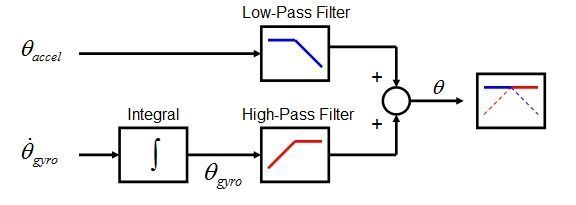
\includegraphics[width=15cm]{pictures/complementary.jpg}
	\caption{Schéma Komplementárního filtru}
	\cite{complementary}
\end{figure}
\begin{eqnarray*} 
	pitch & = & 0.996 * (pitch + xGyro * dt) + 0.004 * pitchAcc\\
	roll & = & 0.996 * (roll + yGyro * dt) + 0.004 * rollAcc\\
\end{eqnarray*}


\subsection{Kalmanův filtr}
Kalmanův filtr je dynamický filtr, který pracuje s predikcí. Pro výpočet je potřeba stanovit model systému, u kterého bude filtr predikovat stavy. Pokud v oblasti predikovaného stavu najdeme skutečný stav, provede se korekce skutečného stavu a oblast predikovaného stavu bude menší/přesnější. Není-li nalezen skutečný stav v oblasti predikovaného stavu, oblast predikovaného stavu se zvětší a tím se zhorší přesnost výpočtu.\\
Bohužel Kalmanův filtr nemohl být použit z důvodu malého výpočetního výkonu platformy Arduino.

\subsection{Mahonyho filtr}
Mahonyho filtr využívá Quaternions, což je čtyř dimenzionální numerický systém využívaný pro popis rotace objektu v počítačové grafice a robotice. Filtr používá data z gyroskopu, akcelerometru a magnetometru, přičemž z nich počítá úhly pitch, roll a yaw. Při výpočtu byla použita knihovna MahonyAHRS. \cite{mahony}\\
%https://github.com/PaulStoffregen/MahonyAHRS
%https://www.youtube.com/watch?v=zjMuIxRvygQ

\section{PID regulátor pro synchronizaci motorů} 
PID regulátor slouží k regulaci požadovaného stavu v nejkratší době a to pomocí zvyšování a snižování vlivu, který napomáhá dostat se do požadovaného stavu.\\
Názorný příklad:
Požadujeme, aby dron držel stabilní polohu. Chceme, aby úhly pitch a roll z IMU byly nulové. Kdybychom měli ideální dron s přesným vyvážením hmotnosti a se stejně fungujícími motory, bylo by to snadné. Pouze by stačilo zapsat stejnou hodnotu na všech motorech a dron by bez problémů vzlétnul. Bohužel ideální dron nemáme, proto motory musí být ovládany individuálně. PID regulátor počítá výkon motoru v závislosti na rozdílu skutečných úhlů od požadovaných.\\
PID regulátor reaguje na tzv. errory (odchylky od požadovaného stavu) a následně přes koeficienty kp, ki a kd spočte hodnoty pro ovládání motorů.
PID regulátor má tři složky: proporcionální (kp), integrační (ki) a derivační (kd).\\
Proporcionální složka ovlivňuje výkon motoru lineárně. Pokud existuje odchylka zvýší se výkon motorů. Pokud je odchylka nulová, proporcioální složka neovlivňuje výkon motorů.\\
Integrační složka ovlivňuje výkon motorů v závislosti na předchozím stavu. Pokud dron není v požadovaném stavu, integrační složka se zvyšuje, dokud není dosažen požadovaný stav.\\
Derivační složka reaguje na změnu rychlosti odchylky. Čím rychleji se bude odchylka měnit, tím větší bude vliv derivační složky. Derivační složka reaguje proti P a I složce.\\
Pro autonomní řízení dronu je potřeba celkem šest PID regulátorů viz obr. 5.7. Základem jsou tři PID regulátory pro úhly pitch, roll a yaw. S těmito třemi regu\-látory, lze létat s dronem přes manuální ovládání. Kontrolu  nad těmito regulátory obstarává letový kontrolér (flying controller).\\
Navigační kontrolér (navigation controller) ovládá další tři regulátory. PID regulátor výkonu (throttle) reaguje na nadmořskou výšku dronu, reguluje konstatní výkon všech motorů pro let ve výšce zadané uživatelem. PID regulátory pro roll a pitch korigují směr letu dronu v závislosti na jeho poloze měřenou GNSS aparaturou.\cite{pid} \cite{hacksterpid}\\
\begin{figure}[H]
	\centering
	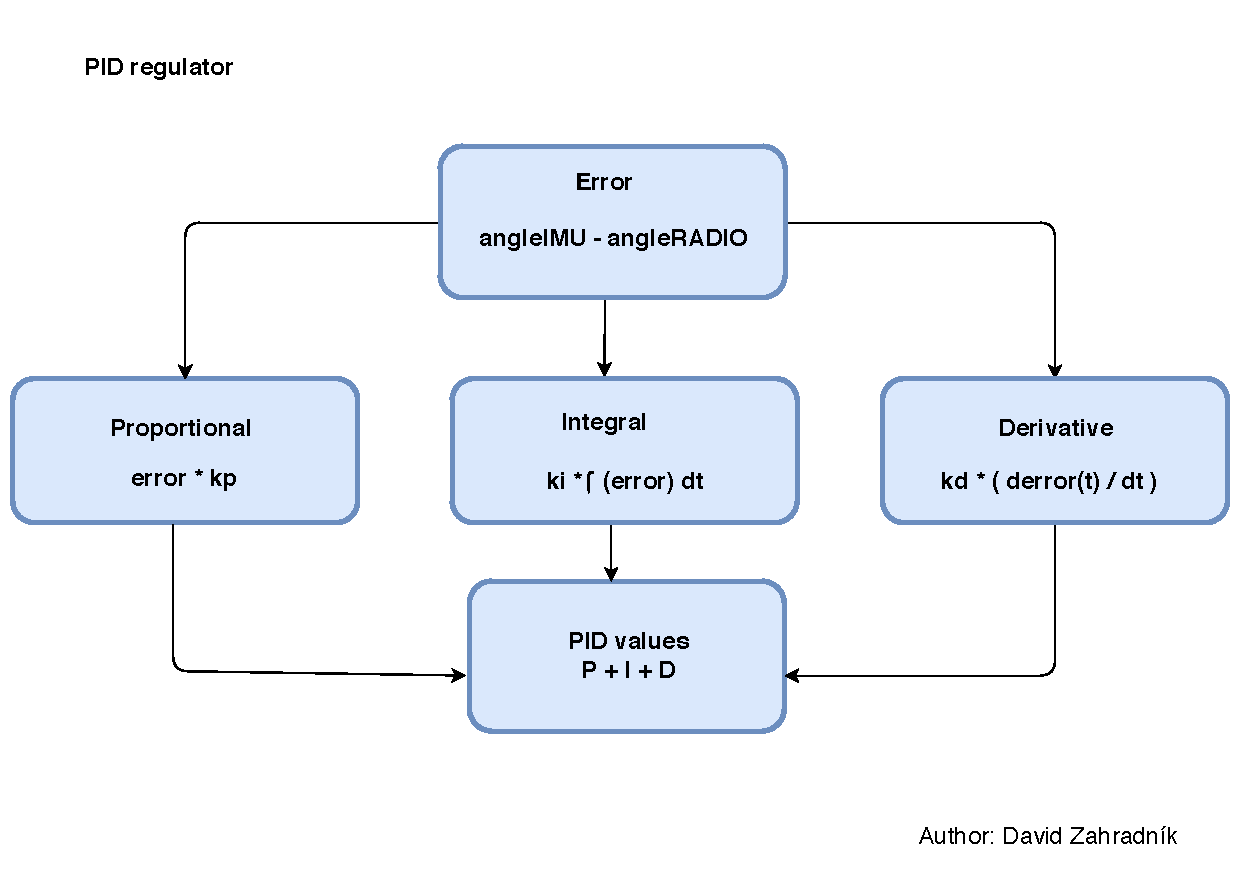
\includegraphics[width=15cm]{pictures/PIDDiagram.pdf}
	\caption{Schéma PID regulátoru}
\end{figure}
\begin{figure}[H]
	\centering
	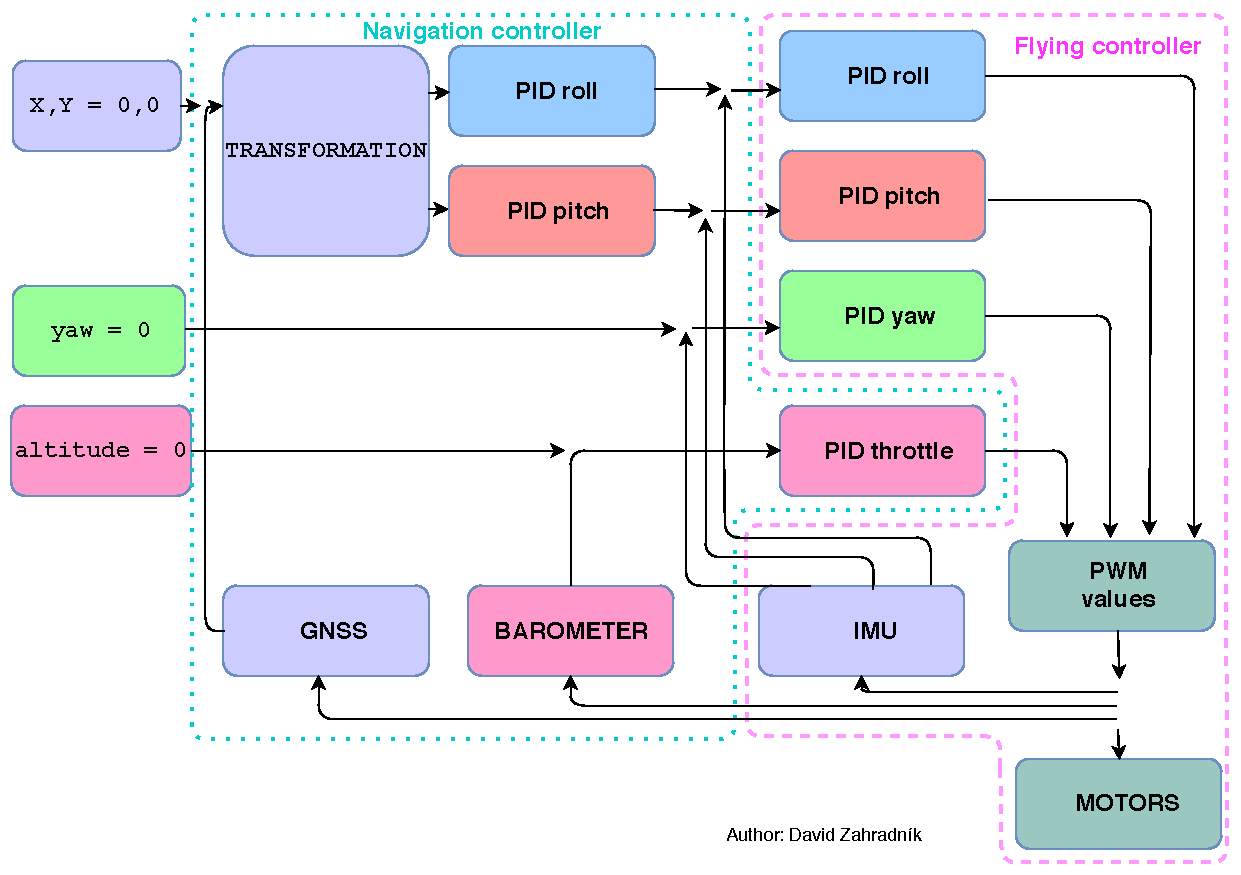
\includegraphics[width=15cm]{pictures/PIDsDiagram.pdf}
	\caption{Schéma všech PID regulátorů při stavbě dronu}
\end{figure}
%https://valter.byl.cz/plynula-regulace-pid
%pid
%http://www.controlengcesko.com/hlavni-menu/artykuly/artykul/article/derivacni-slozka-v-regulaci-pid/

\section{Komunikační protokol}
Pro propojení dronu a smartphonu je použita bluetooth a radiová komunikace. Komunikace je realizována přes sériové rozhraní UART, pro projení se používají piny RX a TX. UART lze implementovat pouze mezi dvěma zařízeními. Pro realizaci komunikace je nutné nastavit stejnou rychlost komunikace (bps).\\
Pro použití rozhraní UART byl vytvořen komunikační protokol pro ovládání dronu. Začátek zprávy je definován znakem < a konec zprávy >. Hodnoty potřebné pro ovládání jsou určeny prvním bytem (znakem) a hodnota následující dvěma byty. Hodnota dána čísly 0-99 se interpoluje do rozsahu uvedeného v tabulce.\\

\begin{table}[H]
	\centering
	\begin{tabular}{|l|l|l|l|}
		\hline
		\textbf{Znak} & \textbf{Typ hodnoty} & \textbf{Od} & \textbf{Do} \\ \hline
		T             & Výkon                & 1000 µS     & 1700 µS     \\ \hline
		P             & Pitch                & -25 $^\circ$        & +25 $^\circ$        \\ \hline
		R             & Roll                 & -25 $^\circ$        & +25 $^\circ$        \\ \hline
		Y             & Yaw                  & 0 $^\circ$          & 360 $^\circ$        \\ \hline
		D             & Stupně               & 48 (12) $^\circ$    & - 52 (15) $^\circ$  \\ \hline
		M             & Minuty               & 0 ´           & 60 ´         \\ \hline
		S             & Sekundy              & 0 ´´          & 60 ´´         \\ \hline
		C             & kalibrace            & null        & null        \\ \hline
		H             & návrat               & null        & null        \\ \hline
		F             & zem. šířka           & null        & null        \\ \hline
		L             & zem. délka           & null        & null        \\ \hline
	\end{tabular}
\caption{Komunikační protokol přes seriové rozhraní UART}
\end{table}

\section{Radiová komunikace XBEE}
Před zahájením komunikace mezi radiovými moduly je nutné provést jejich konfi\-guraci. Ke konfiguraci slouží program XCTU (Linux, Windows) od výrobců mo\-dulů XBEE. Pro propojení počítače a modulu lze použít shield (nadstavbové zařízení k mikrokontrolérům) od firmy Digi, nebo je možné využít platformu Arduino a \mbox{Arduino} XBEE shield.\\
K propojení radiového modulu a počítače s pomocí platformy Arduino, je nutno provést několik kroků. V první řadě je do platformy nahrán jednoduchý kód, který bude mít za úkol číst data z počítače a posílat je radiovému modulu. V kódu je třeba definovat, na kterých pinech bude prováděna komunikace s radiovým mo\-dulem. Druhý krok je nastavení pinů pro komunikaci s radiovým modulem na shieldu. V posledním kroku jsou dílčí součástky spojeny.\\
Nejdůležitějšími nastaveními radiových modulů jsou definování funkce, rychlost komunikace (bps) a ID sítě. V síti radiových modulů je potřeba jeden koordinátor, na počtu routerů a koncových zařízení nezáleží. Koordinátor obstarává inicializaci sítě a umožnuje dalším modulům připojení do sítě. Router funguje jako prostředník při přenosu dat. Koncové zařízení slouží buď k příjmu nebo odesílání zpráv. Rychlost komunikace je dána přenosem bitů za sekundu (bps) a musí být totožná na všech zařízeních v síti. ID sítě slouží k uzavření komunikace jenom mezi určitými radiovými moduly. \cite{xbeetut}\\\\
%https://www.tunnelsup.com/xbee-guide/
%xbeetut

\begin{figure}[H]
	\centering
	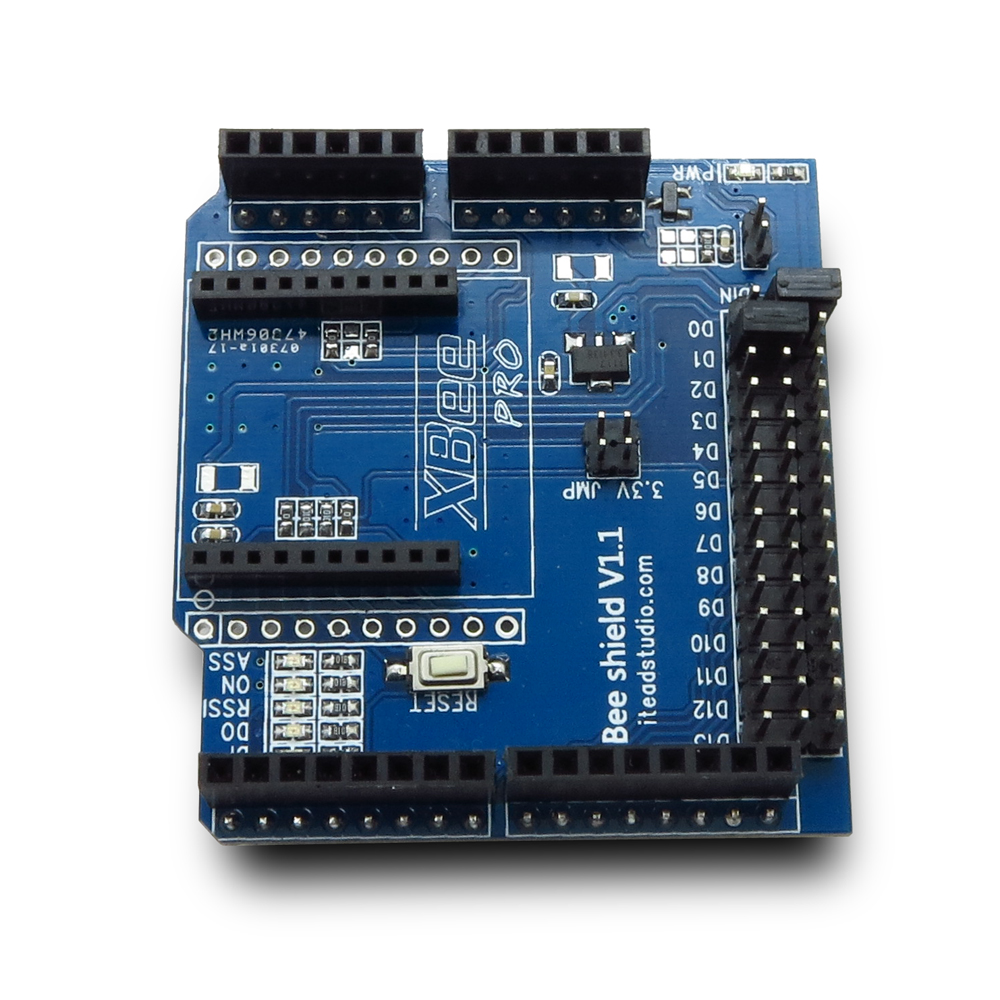
\includegraphics[width=8cm]{pictures/xbeeshield.jpg}
	\caption{XBEE shield}
\end{figure}


\section{Letový kontrolér} 
\textbf{Vstup:} IMU, Navigační kontrolér\\
\textbf{Výstup:} ESC\\
Letový kontrolér slouží k synchronizaci a ovládání motorů dronu. Letový kontrolér zpracovává měření z IMU a porovnává jej s daty z navigačního kontroléru (pitch, roll a yaw). Pokud úhly náklonů nejsou totožné, kontrolér přes PID regulátory změní výkon motorů tak, aby úhly ztotožnil.\\
Při spuštění letový kontrolér provede kalibraci regulátorů otáček zapsáním minimální a maximální hodnoty výkonu.\\
Po kalibraci regulátorů otáček, kontrolér čte data z IMU, probíhá filtrace pomocí komplementárního filtru a počítá úhly pitch, roll a yaw.\\
Z navigačního kontroléru jsou získávána data, která jsou následně separována a interpolována do požadovaných hodnot. Hodnoty jsou rozlišovány prvním bytem, který definuje o jakou hodnotu se jedná. Další dva byty představují číslo od 0 do 99, které je interpolováno na požadovaný rozsah.\\
Hodnota výkonu motoru/throttle se vyinterpoluje pouze do 1700 µS, protože ke konstantnímu výkonu jsou připočítávány údaje z PID regulátoru. Rozsah dat z PID regulátoru je <-300;300>, pokud by se zapsal konstaní výkon větší než 1700 µS, PID regulátor by byl omezen.\\
Hodnota náklonů pitch a roll  může být nejvýše 25 stupňů, kdyby byla hodnota větší, hrozilo by převrácení dronu.\\
Z rozdílu úhlů z IMU a navigačního kontroléru se vypočtou odchylky. Podle odchylek se vyčíslí proporcionální, integrační a derivační složka PID regulátoru každého úhlu. Součet všech tři složek představuje změnu výkonu motoru pro jednotlivý úhel. Dle pohybových rovnic jsou vypočteny výkony motorů.\\
Pro zápis výkonu motorů byl implementován komunikční protokol s frekvencí 250 Hz(viz obrázek 5.10), který výchází ze standartního PWM signálu. První fázi je prováden výpočet komplementárního filtru, výpočet hodnot PID regulátorů a čtení dat za navigačního kontroléru. Ve druhé fázi jsou čtena data z IMU jednotky a zapisovány hodnoty výkonu pro regulátory otáček(ESC). Doba trvání obou fázi jsou čtyči milisekundy, frekvence tedy je 250 Hz. V druhé fázi, kdy zapisování hodnot výkonu trvá jednu až dvě milisekundy, jsou pro úsporu času v první milisekundě čtena data z IMU jednotky.\\
\begin{figure}[H]
	\centering
	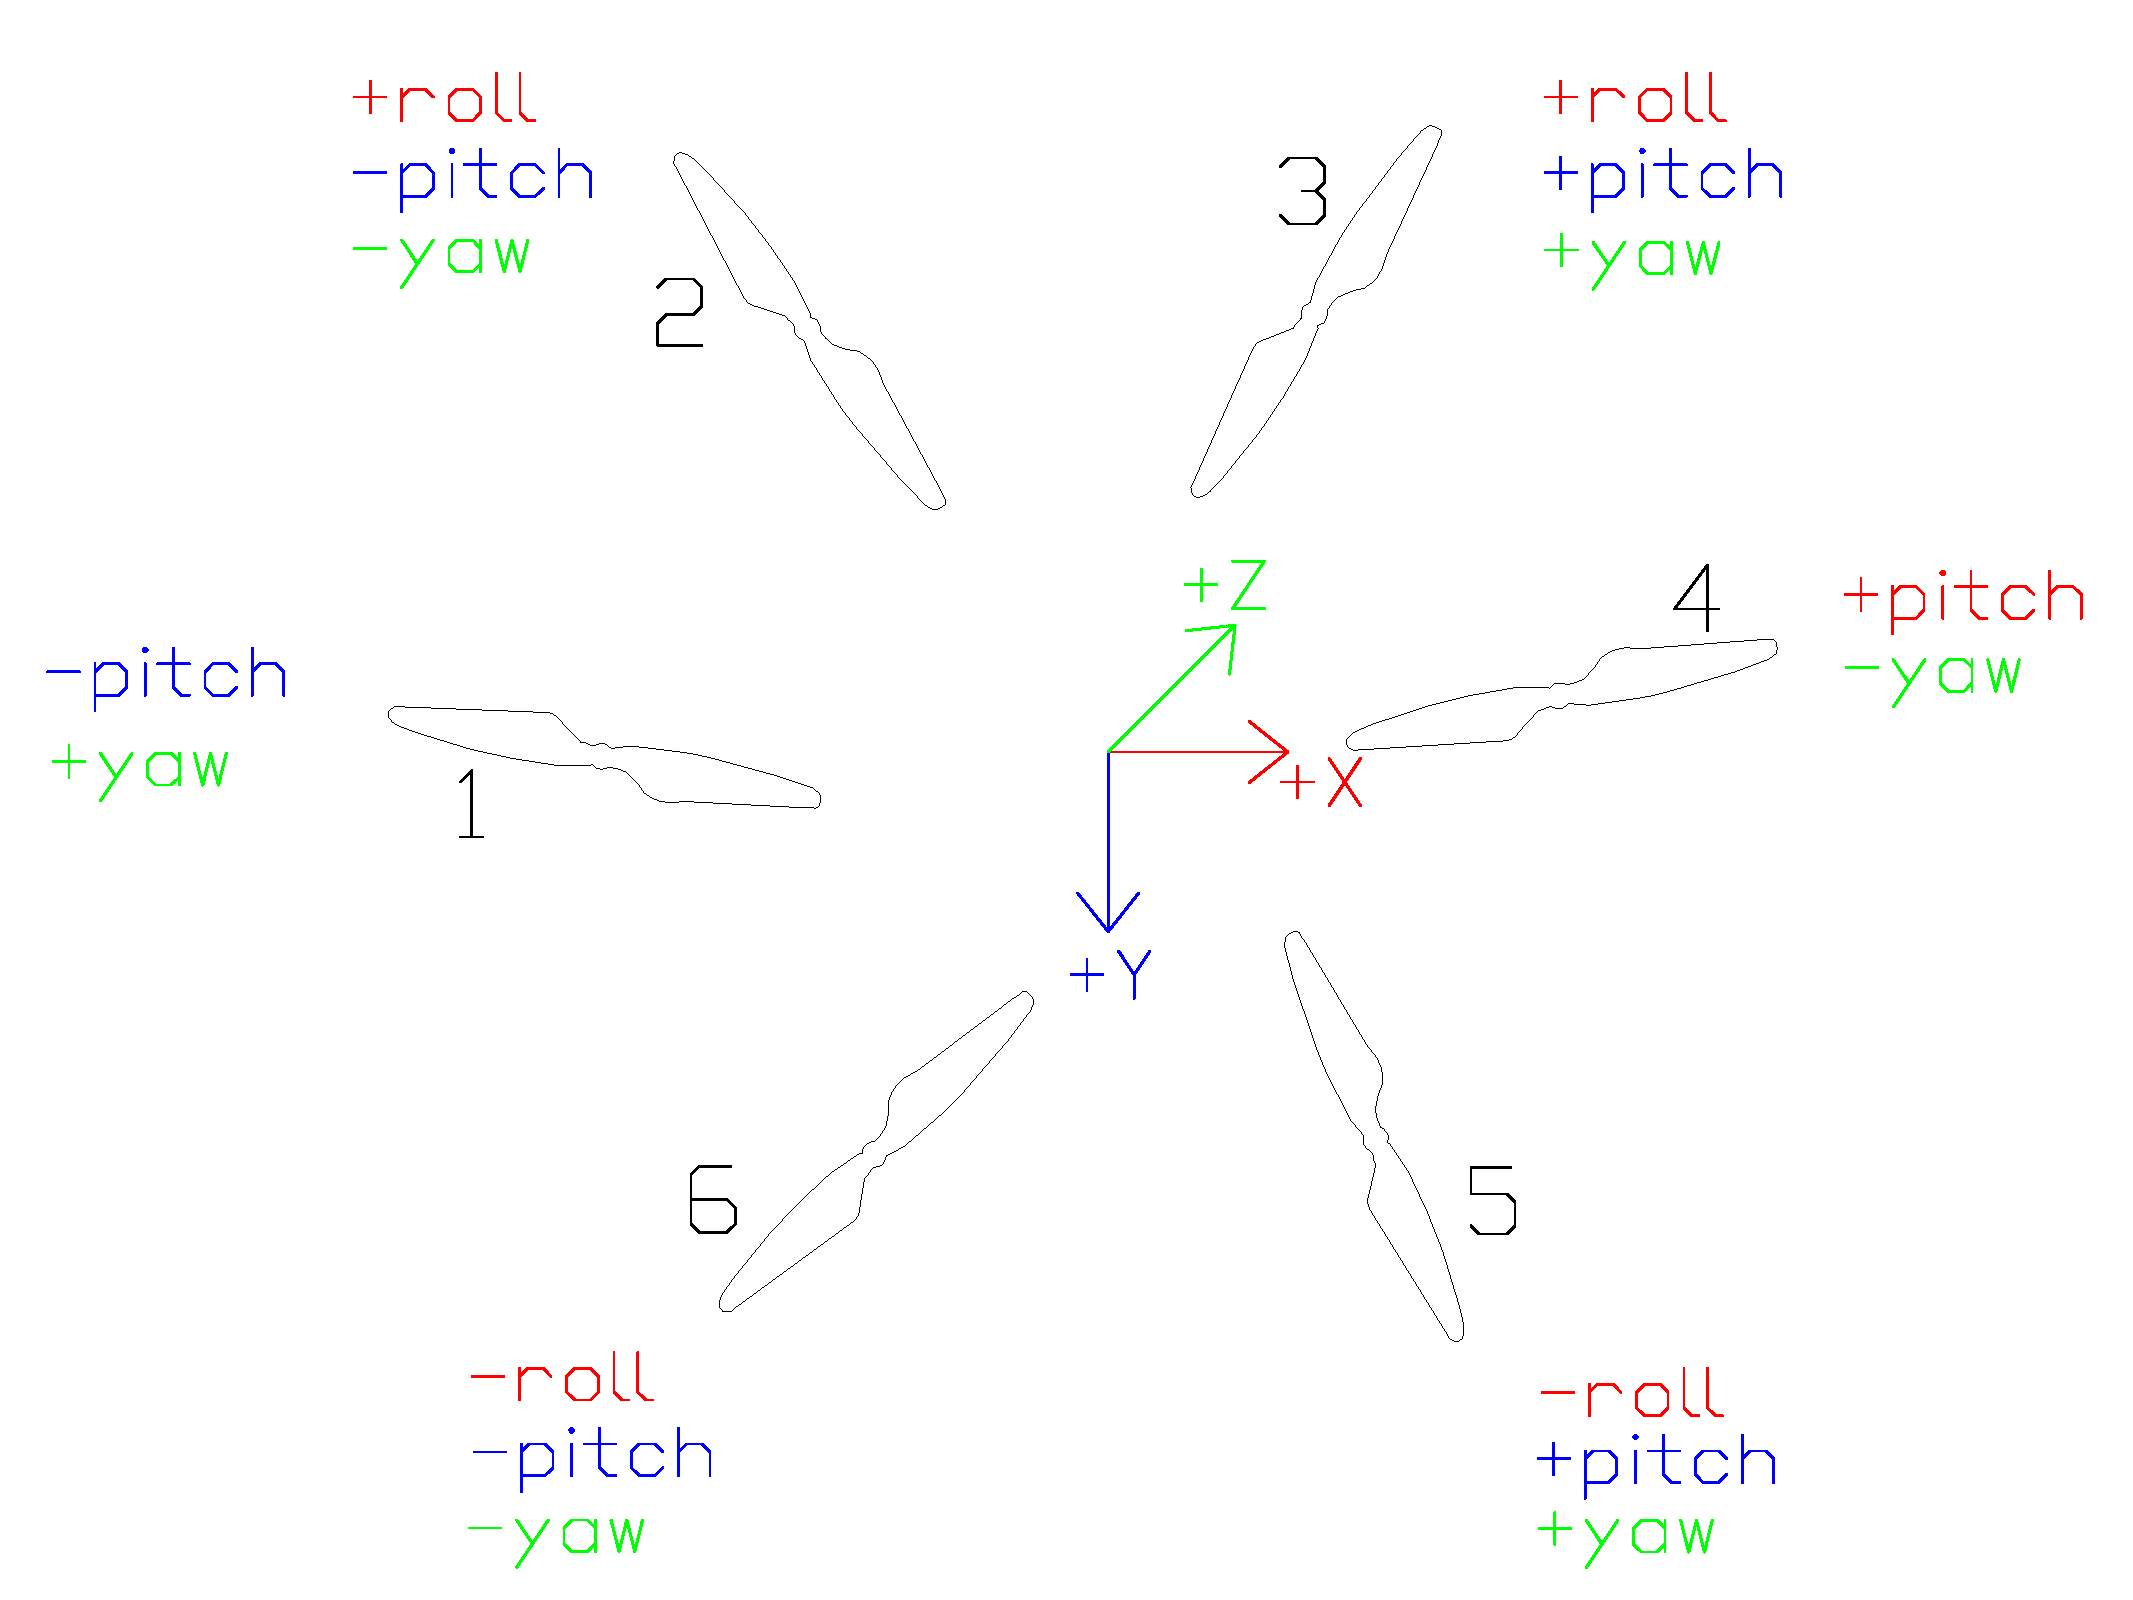
\includegraphics[width=9cm]{pictures/pid.pdf}
	\caption{Schéma ovládání dronu podle úhlu náklonu}
\end{figure}
\textbf{Pohybové rovnice}
\begin{eqnarray*} 
	motor1 & = & throttle - pidPitch           + pidYaw\\
	motor2 & = & throttle - pidPitch + pidRoll - pidYaw\\
	motor3 & = & throttle + pidPitch + pidRoll + pidYaw\\
	motor4 & = & throttle + pidPitch           - pidYaw\\
	motor5 & = & throttle + pidPitch - pidRoll + pidYaw\\
	motor6 & = & throttle - pidPitch - pidRoll - pidYaw\\
\end{eqnarray*} 

\begin{figure}[H]
	\centering
	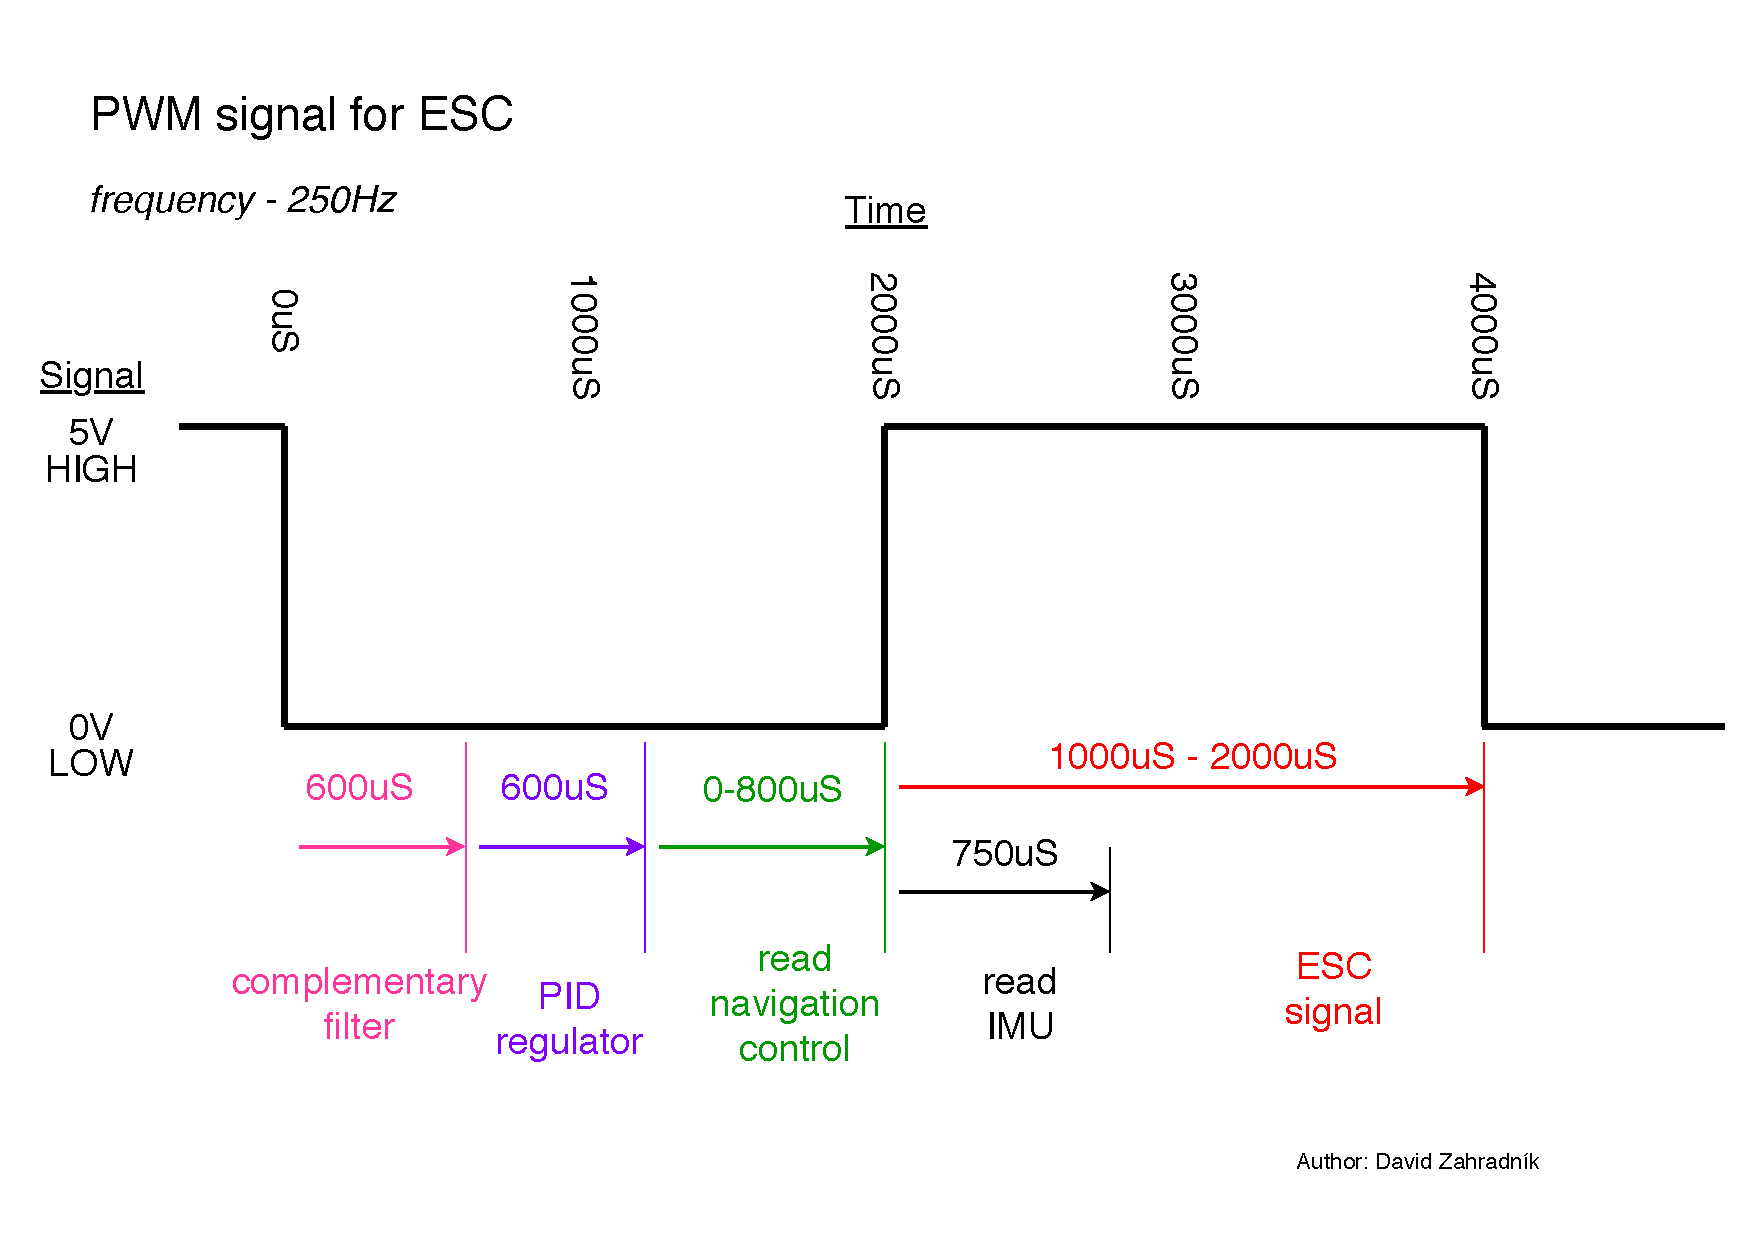
\includegraphics[width=16cm]{pictures/PWMDiagram.pdf}
	\caption{Diagram PWM signálu}
\end{figure}
\begin{figure}[H]
	\centering
	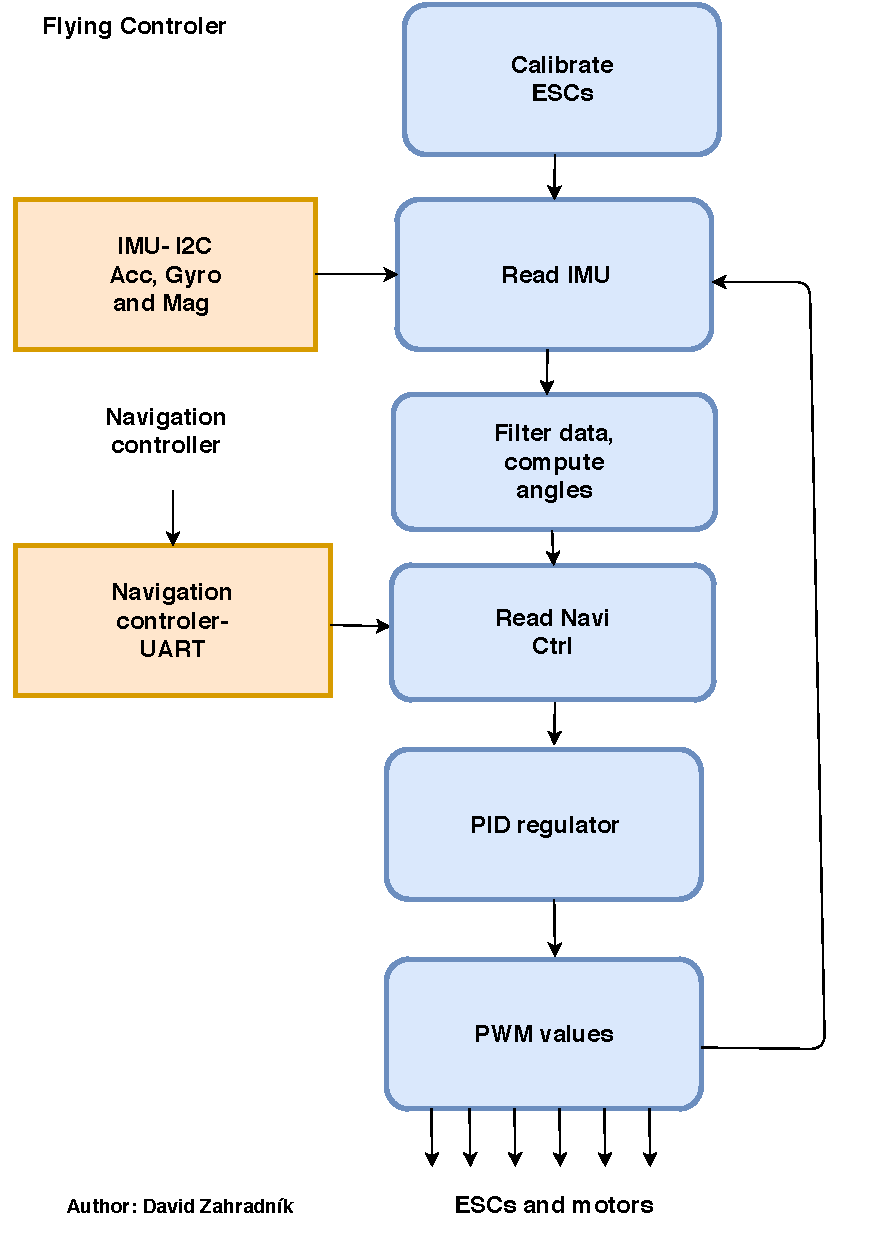
\includegraphics[width=12cm]{pictures/FlyingDiagram.pdf}
	\caption{Diagram algoritmu letového kontroléru}
\end{figure}
\begin{figure}[H]
	\centering
	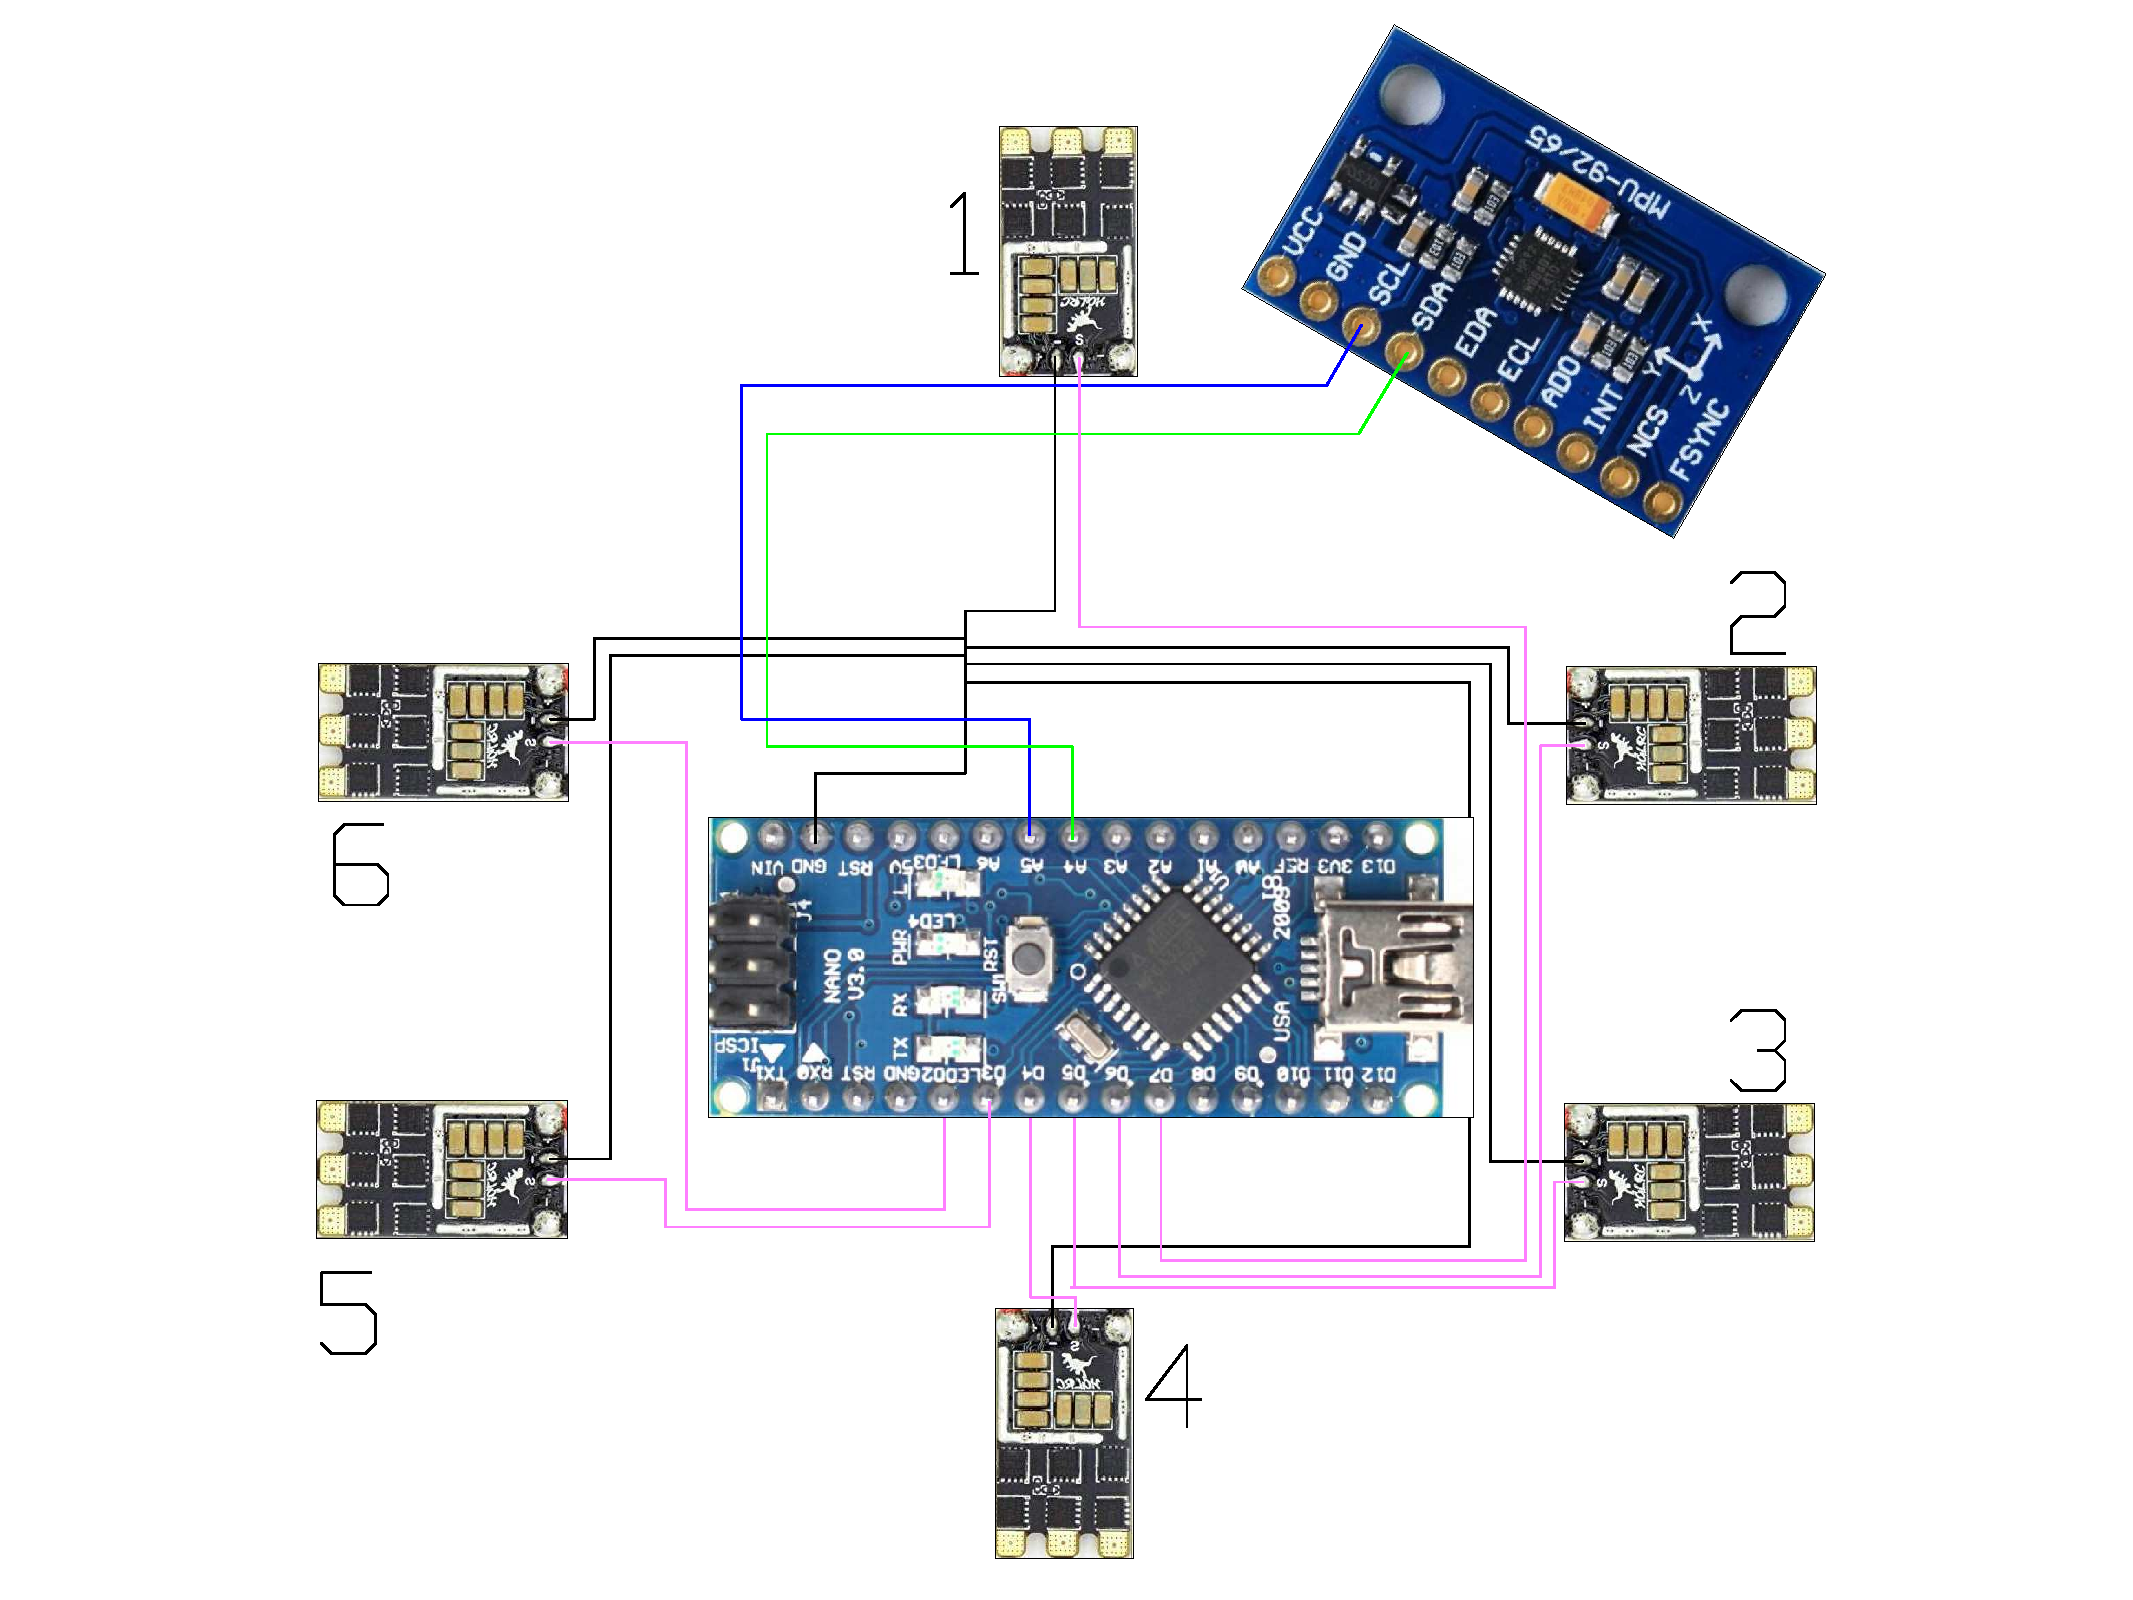
\includegraphics[width=12cm]{pictures/flyctrl.pdf}
	\caption{Schéma zapojení letového kontroléru}
\end{figure}

\section{Překážkový kontrolér} 
\textbf{Vstup:} 7x laserový modul\\
\textbf{Výstup:} Navigační kontrolér\\
Překážkový kontrolér upozorňuje navigační kontrolér o existenci cizího objektu v okolí dronu. Laserové moduly jsou nasměrovány do směrů pohybu podle úhlů pitch, roll a jeden laser je nasměrován po svislici pro přistávání. Lasery jsou nastaveny na kontinuální měření vzdáleností. Pokud se v blízkosti nachází cizí objekt, kontrolér pošle zprávu o překážce navigačnímu kontroléru a její poloze.\\

\begin{figure}[H]
	\centering
	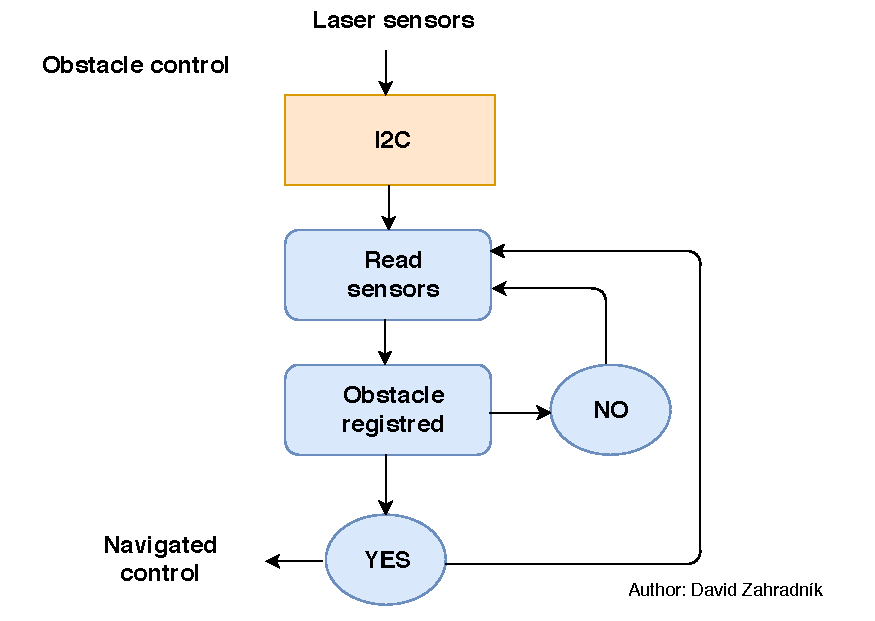
\includegraphics[width=12cm]{pictures/ObstacleDiagram.pdf}
	\caption{Diagram algoritmu překážkového kontroléru}
\end{figure}

\begin{figure}[H]
	\centering
	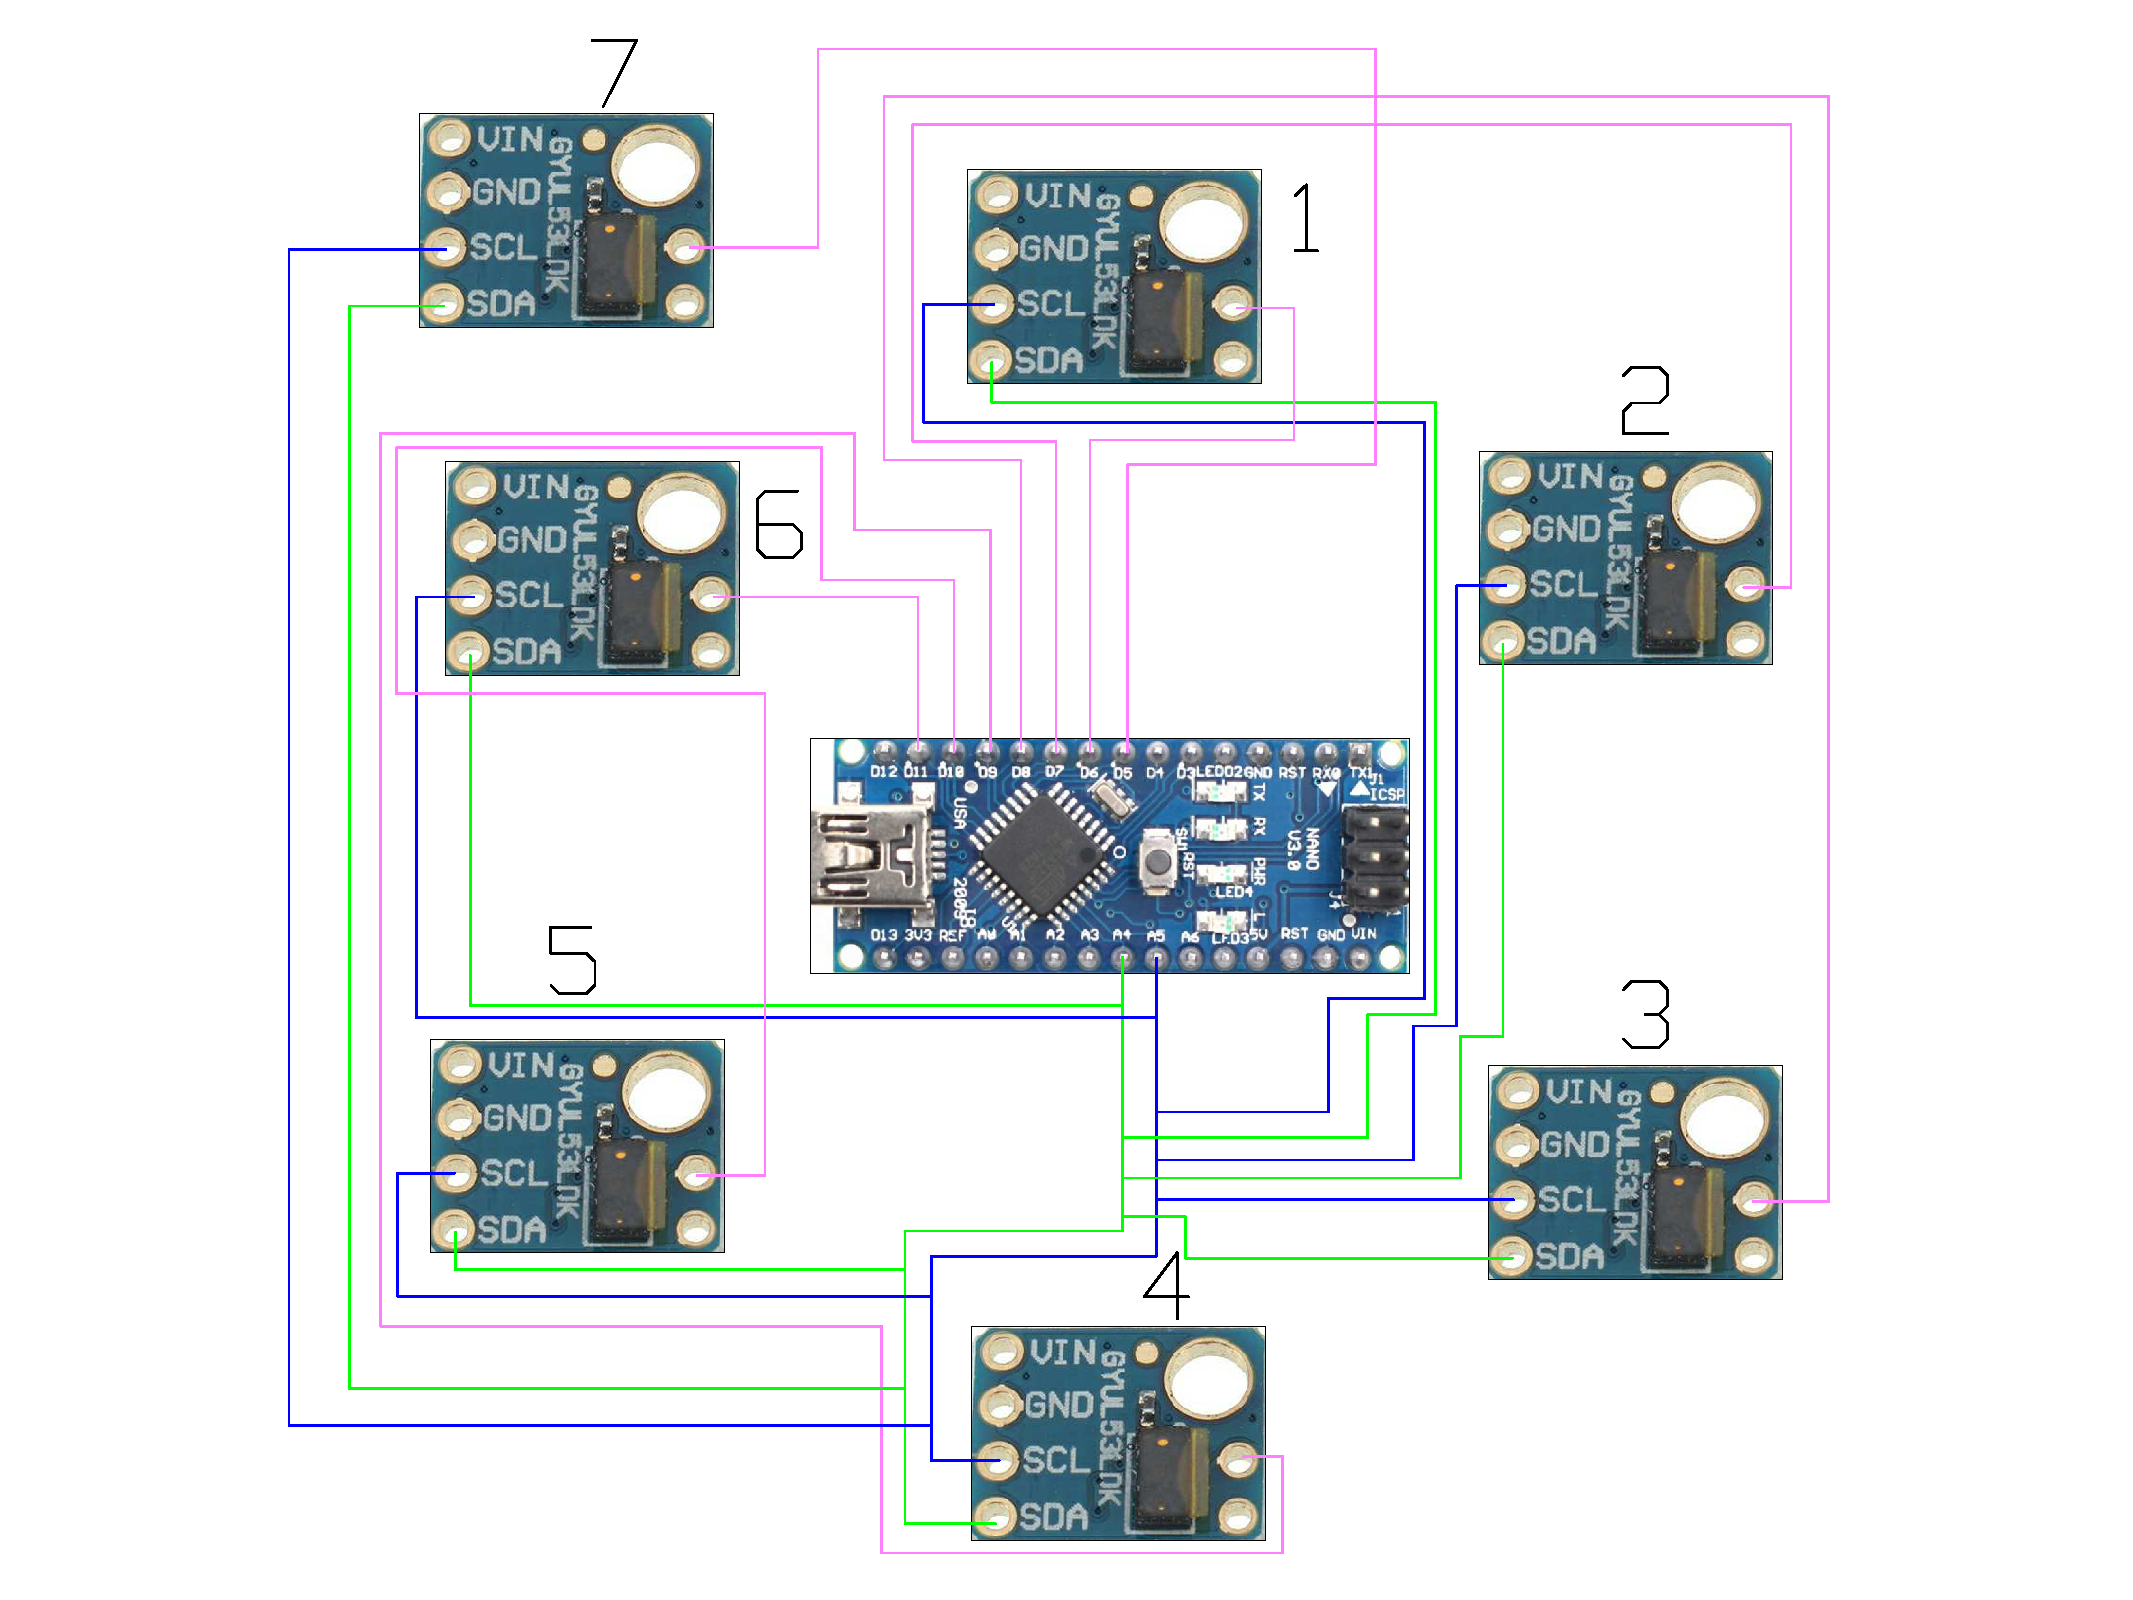
\includegraphics[width=10cm]{pictures/obstacle.pdf}
	\caption{Schéma zapojení Překážkového kontroléru}
\end{figure}

\begin{figure}[H]
	\centering
	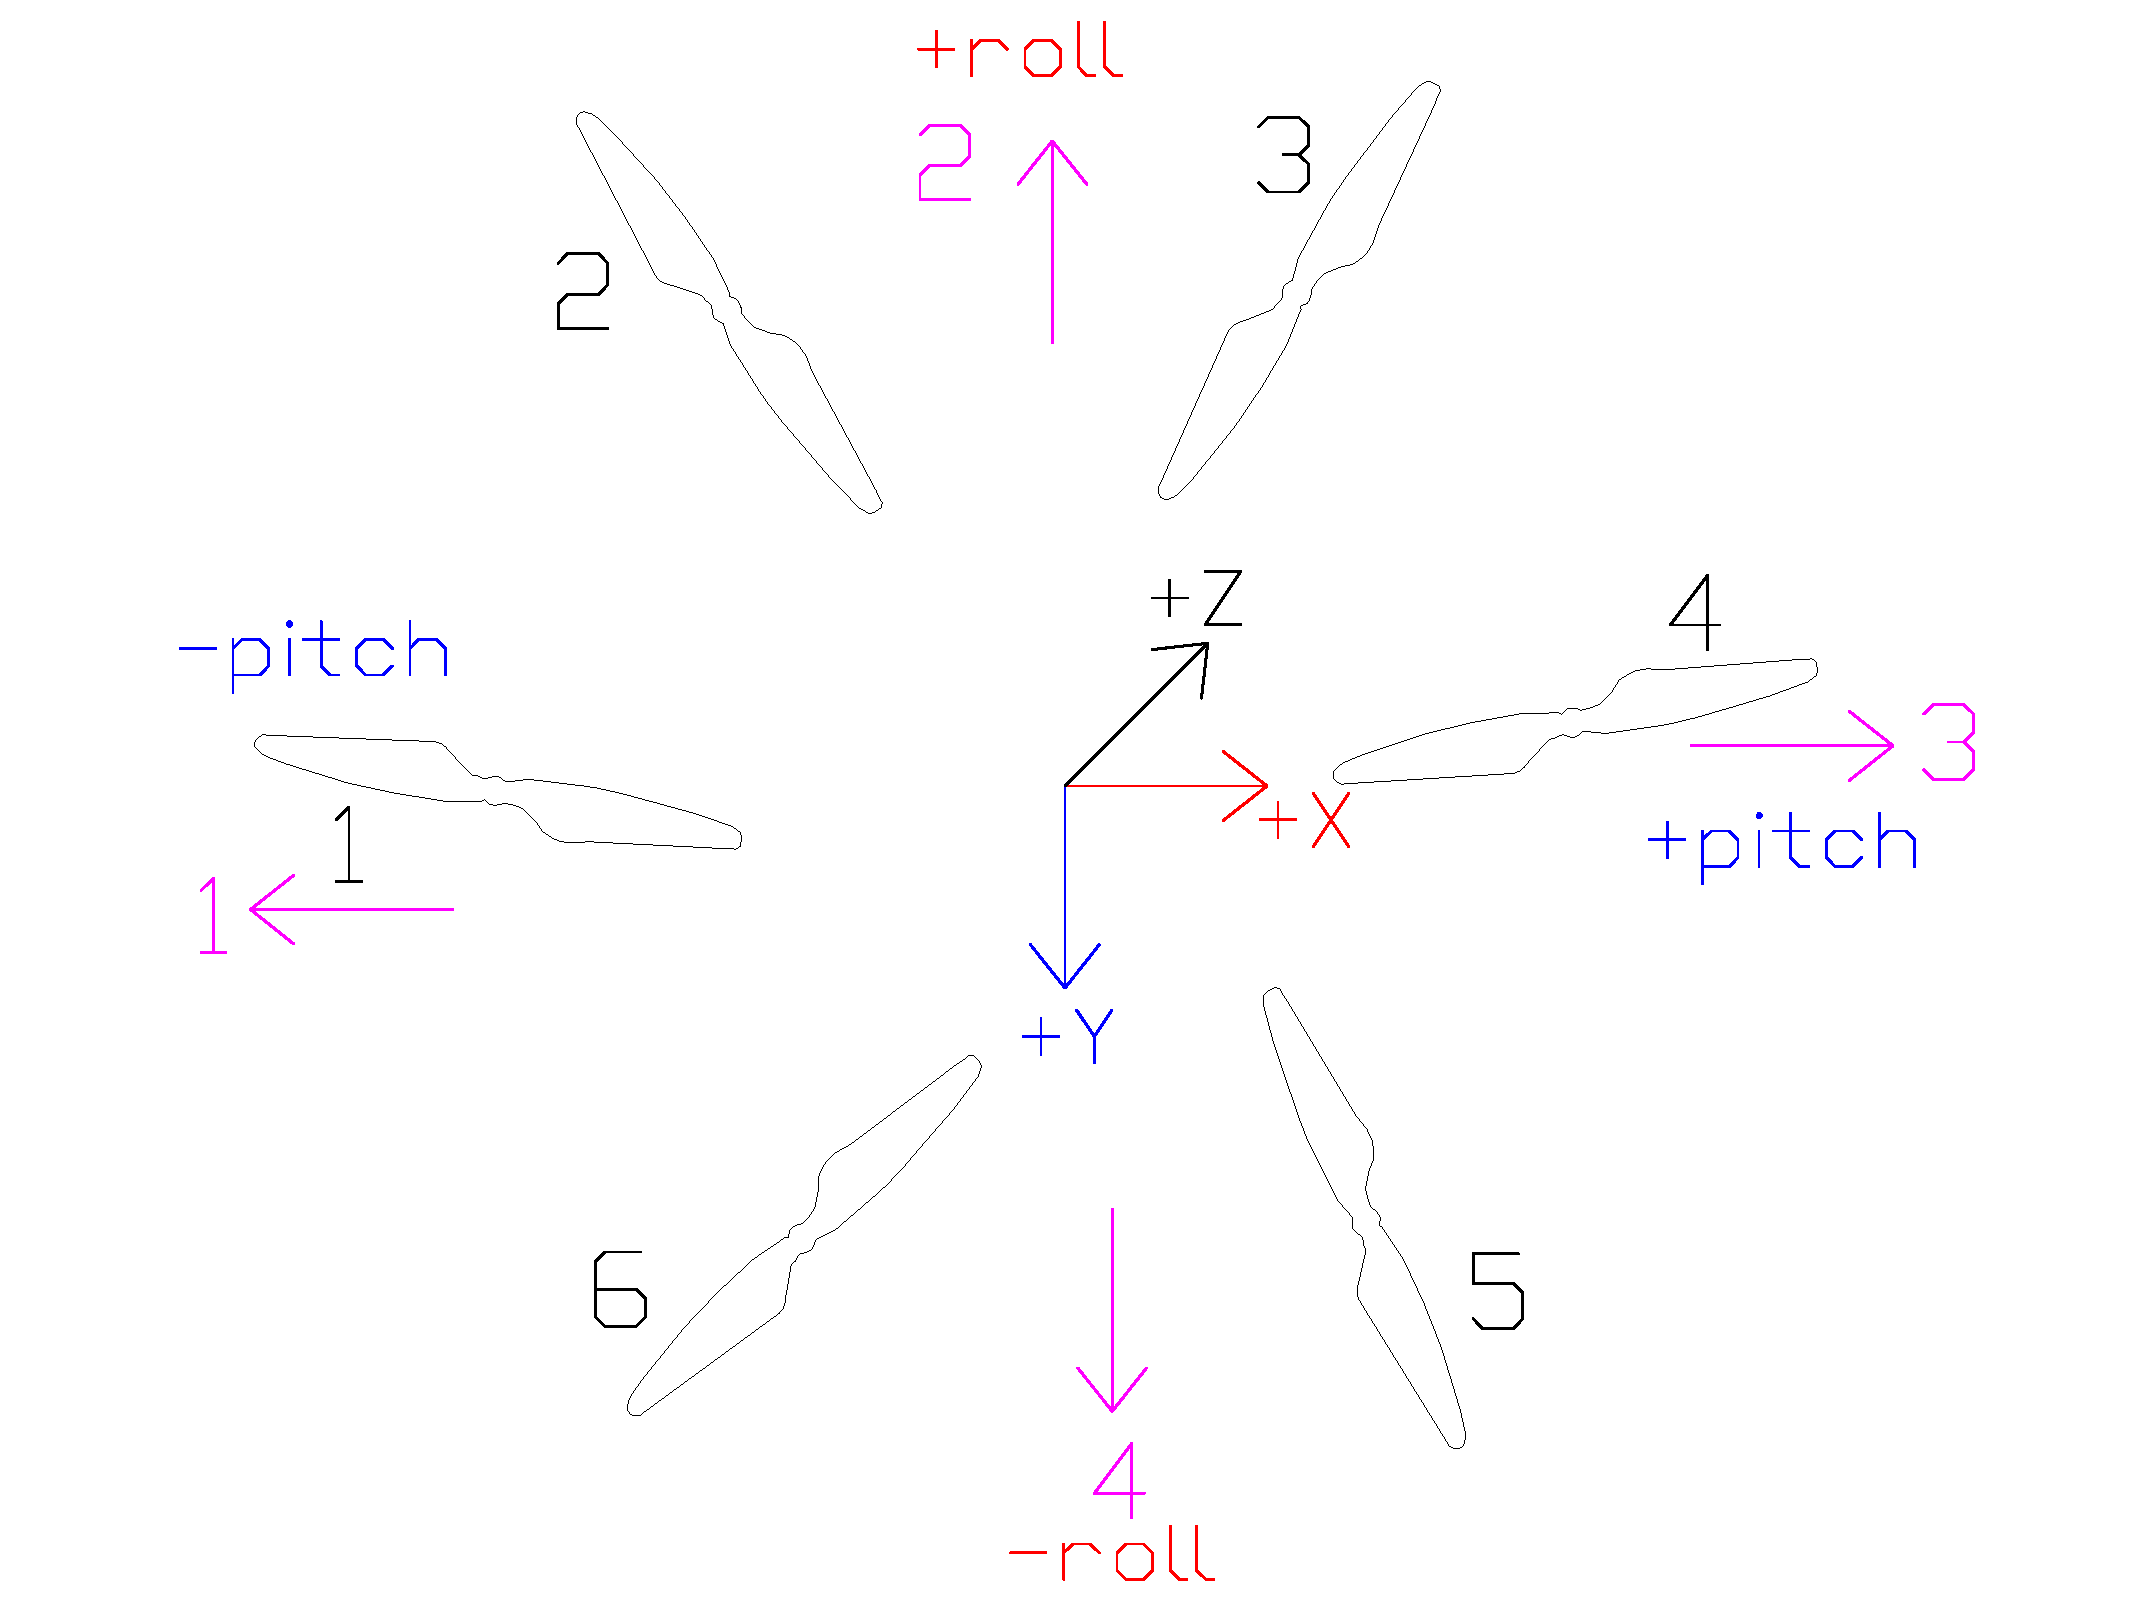
\includegraphics[width=10cm]{pictures/obstacle_teo.pdf}
	\caption{Schéma zpráv o překážce}
\end{figure}

\begin{table}[H]
	\centering
	\begin{tabular}{|l|l|l|}
		\hline
		\textbf{+/-} & \textbf{Úhel} & \textbf{Zpráva} \\ \hline
		+            & roll          & 2               \\ \hline
		-            & roll          & 4               \\ \hline
		-            & pitch         & 3               \\ \hline
		+            & pitch         & 1               \\ \hline
		& down          & 5               \\ \hline
	\end{tabular}
	\caption{Zpráva o překážce}
\end{table}

\section{Navigační kontrolér} 
\textbf{Vstup:} Rádio, Bluetooth, Barometr, GNSS, Překážkový kontrolér\\
\textbf{Výstup:} Letový kontrolér\\
Navigační kontrolér složí ke komunikaci s ovládacím zařízením, sběru dat z gnss, barometru a překážkového kontroléru.\\
Po zapnutí bude kontrolér čekat na zprávu ze smartphonu. Podle typu příchozích dat kontrolér nastaví autonomní nebo manuální řízení.\\
Používá-li uživatel manuální ovládání, navigační kontrolér pouze ověří zda existuje překážka, pokud existuje, zámezí srážce. Neexistuje-li překážka kontrolér pošle data letovému kontroléru.\\
Při autonomním ovládání kontrolér porovná data z GNSS aparatury a zadané souřadnice. Pokud souřadnice nejsou totožné, vypočte se směr a vzdálenost z polohy dronu a zadaných souřadnic. Provede se shodnostní transformace ze souřadnicového systému GNSS aparatury do souřadnicového systému dronu. Vstupní data pro PID regulátor budou souřadnicové rozdíly v souřadnicovém systému dronu a výstupní data budou úhly pitch a roll.\\
Při držení určité nadmořské výšky se zvovu použije PID regulátor. Vstupním datem bude nadmořská výška z GNSS aparatury nebo z barometru, výstupem bude výkon motoru, který bude konstatní pro všechny motory.\\
Bude definována funkce návrat, při které se dron vrátí na startovní místo. Pozice startovního místa bude změřena GNSS aparaturou automaticky před startem dronu.\\

\begin{figure}[H]
	\centering
	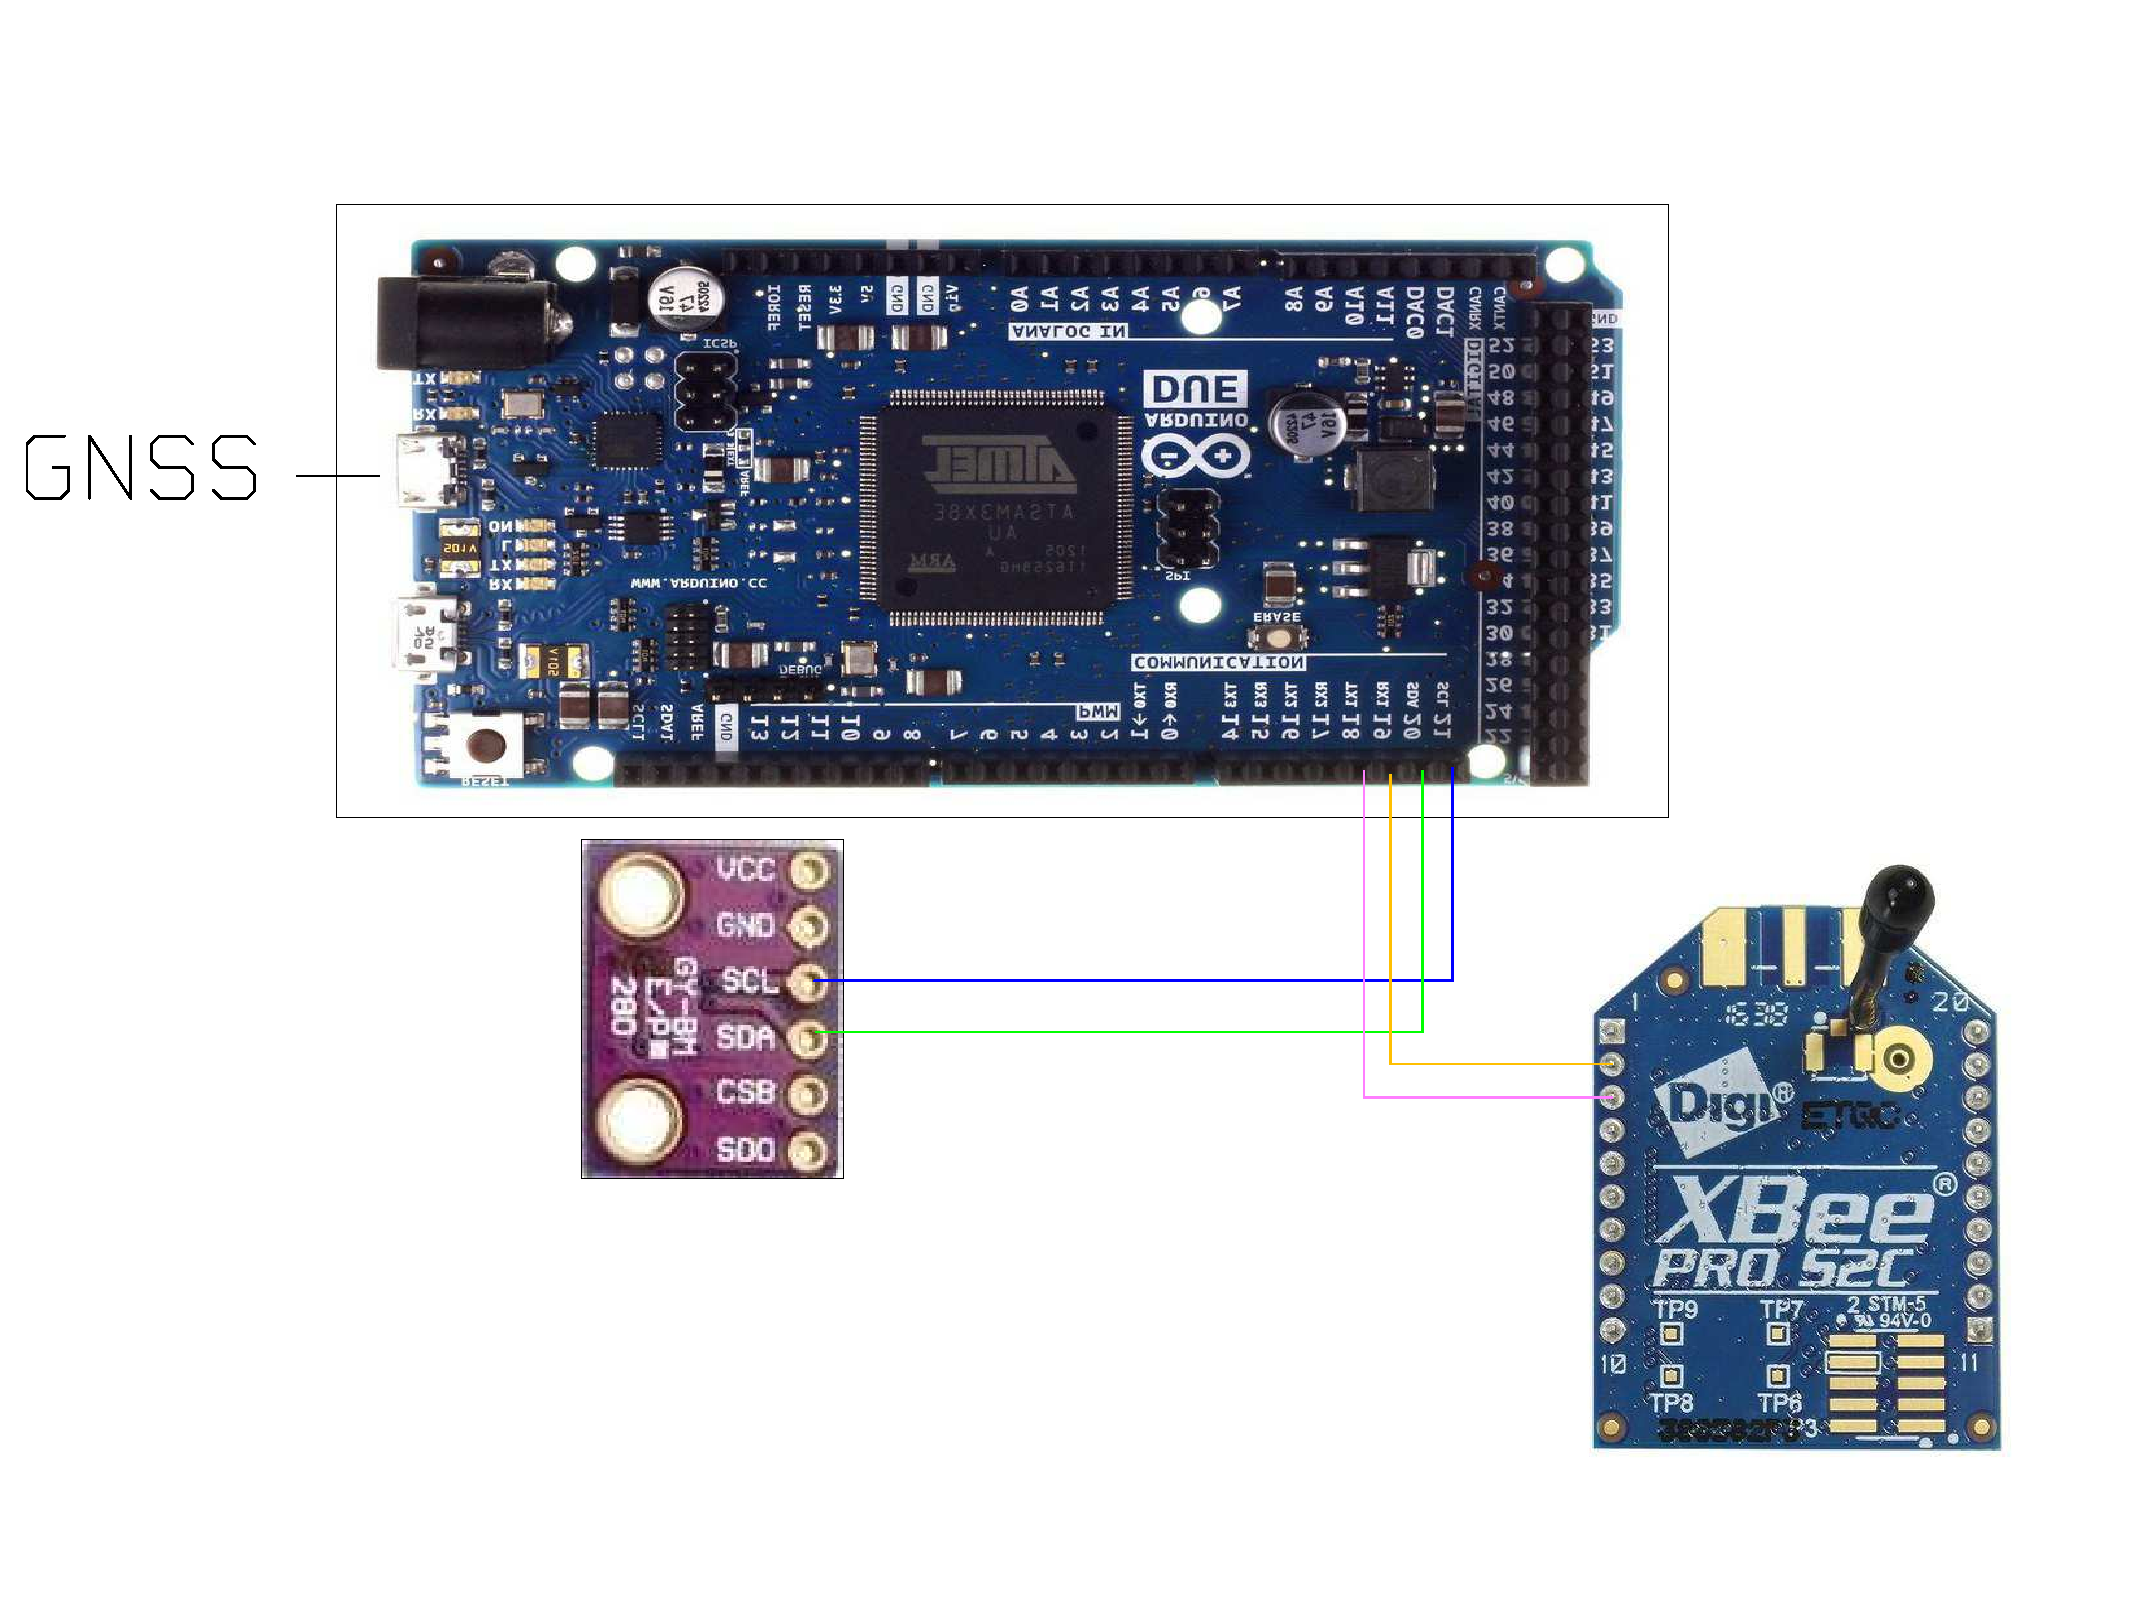
\includegraphics[width=10cm]{pictures/navictrl.pdf}
	\caption{Schéma zapojení Navigačního kontroléru}
\end{figure}
\begin{figure}[H]
	\centering
	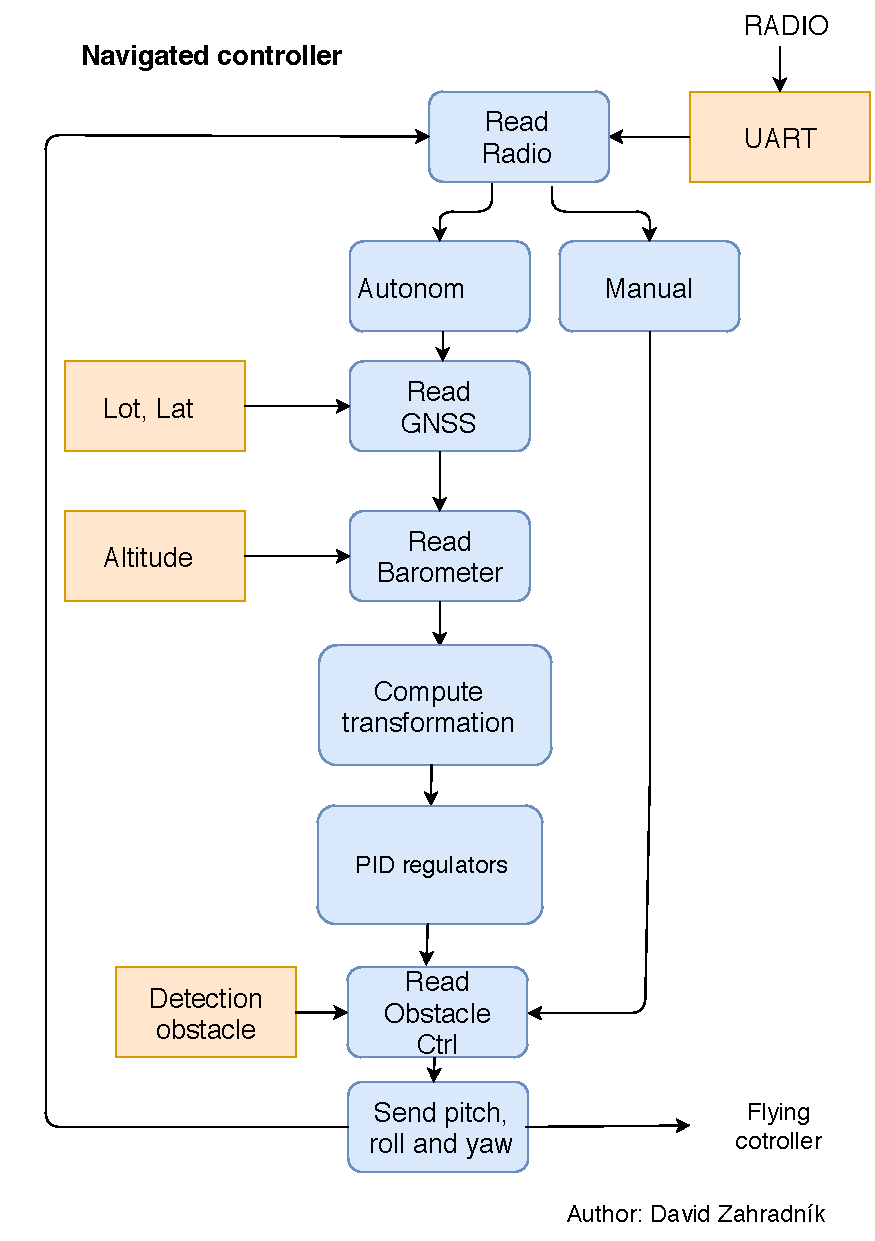
\includegraphics[width=14cm]{pictures/NaviDiagram.pdf}
	\caption{Diagram navigačního kontroléru}
\end{figure}


\section{Finální sestavení}
Z důvodů nízkého výpočetního výkonu platfromy Arduino je komplení ovládání sestaveno ze tří platforem Arduino. Letový kontrolér ovládá jednotlivé motory, překážkový kontrolér detekuje případné překážky a navigační kontrolér komunikuje s ovladačem a řídí let.\\
Distribuční deska s regulátory otáček jsou umístěny ve spodní části dronu pod baterii. Byl zjištěn negativní vliv magnetického pole regulátorů pro ovládací prvky. Magnetické pole bylo tak silné, že ovládací prvky byly neovladatelné. Ovládací prvky jsou umístěné na vrchní části dronu. Barometr a GNSS aparatura jsou vyvýšené nad vrtulemi, aby tlak vzduchu neovlivňoval jejich funkčnost.\\
Dron je ovládán smartphonem přes uzlové zařízení. Uzlové zařízení se skládá z bluetooth a radiového modulu. Tok dat probíhá ze smartphonu přes bluetooth do uzlového zařízení a ze zařízení do navigačního kontroléru přes radiový signál.\\
Kamera posílá data smartphonu nezávisle na ovládání dronu. Kamera obsahuje vlastní radiový vysílač, který vysílá data přijímači připojeného k smartphonu skrze miniUSB. Pro správnou funkci kamery musí smartphone podporovat funkci OTG.\\
Při připevnění IMU jednotky kovovými šrouby na konstrukci dronu, byl zjištěn ne\-gativní vliv kovu na data z IMU, proto všechny řídící komponenty jsou připevněny k nepájivému poli.\\
\begin{figure}[h]
	\centering
	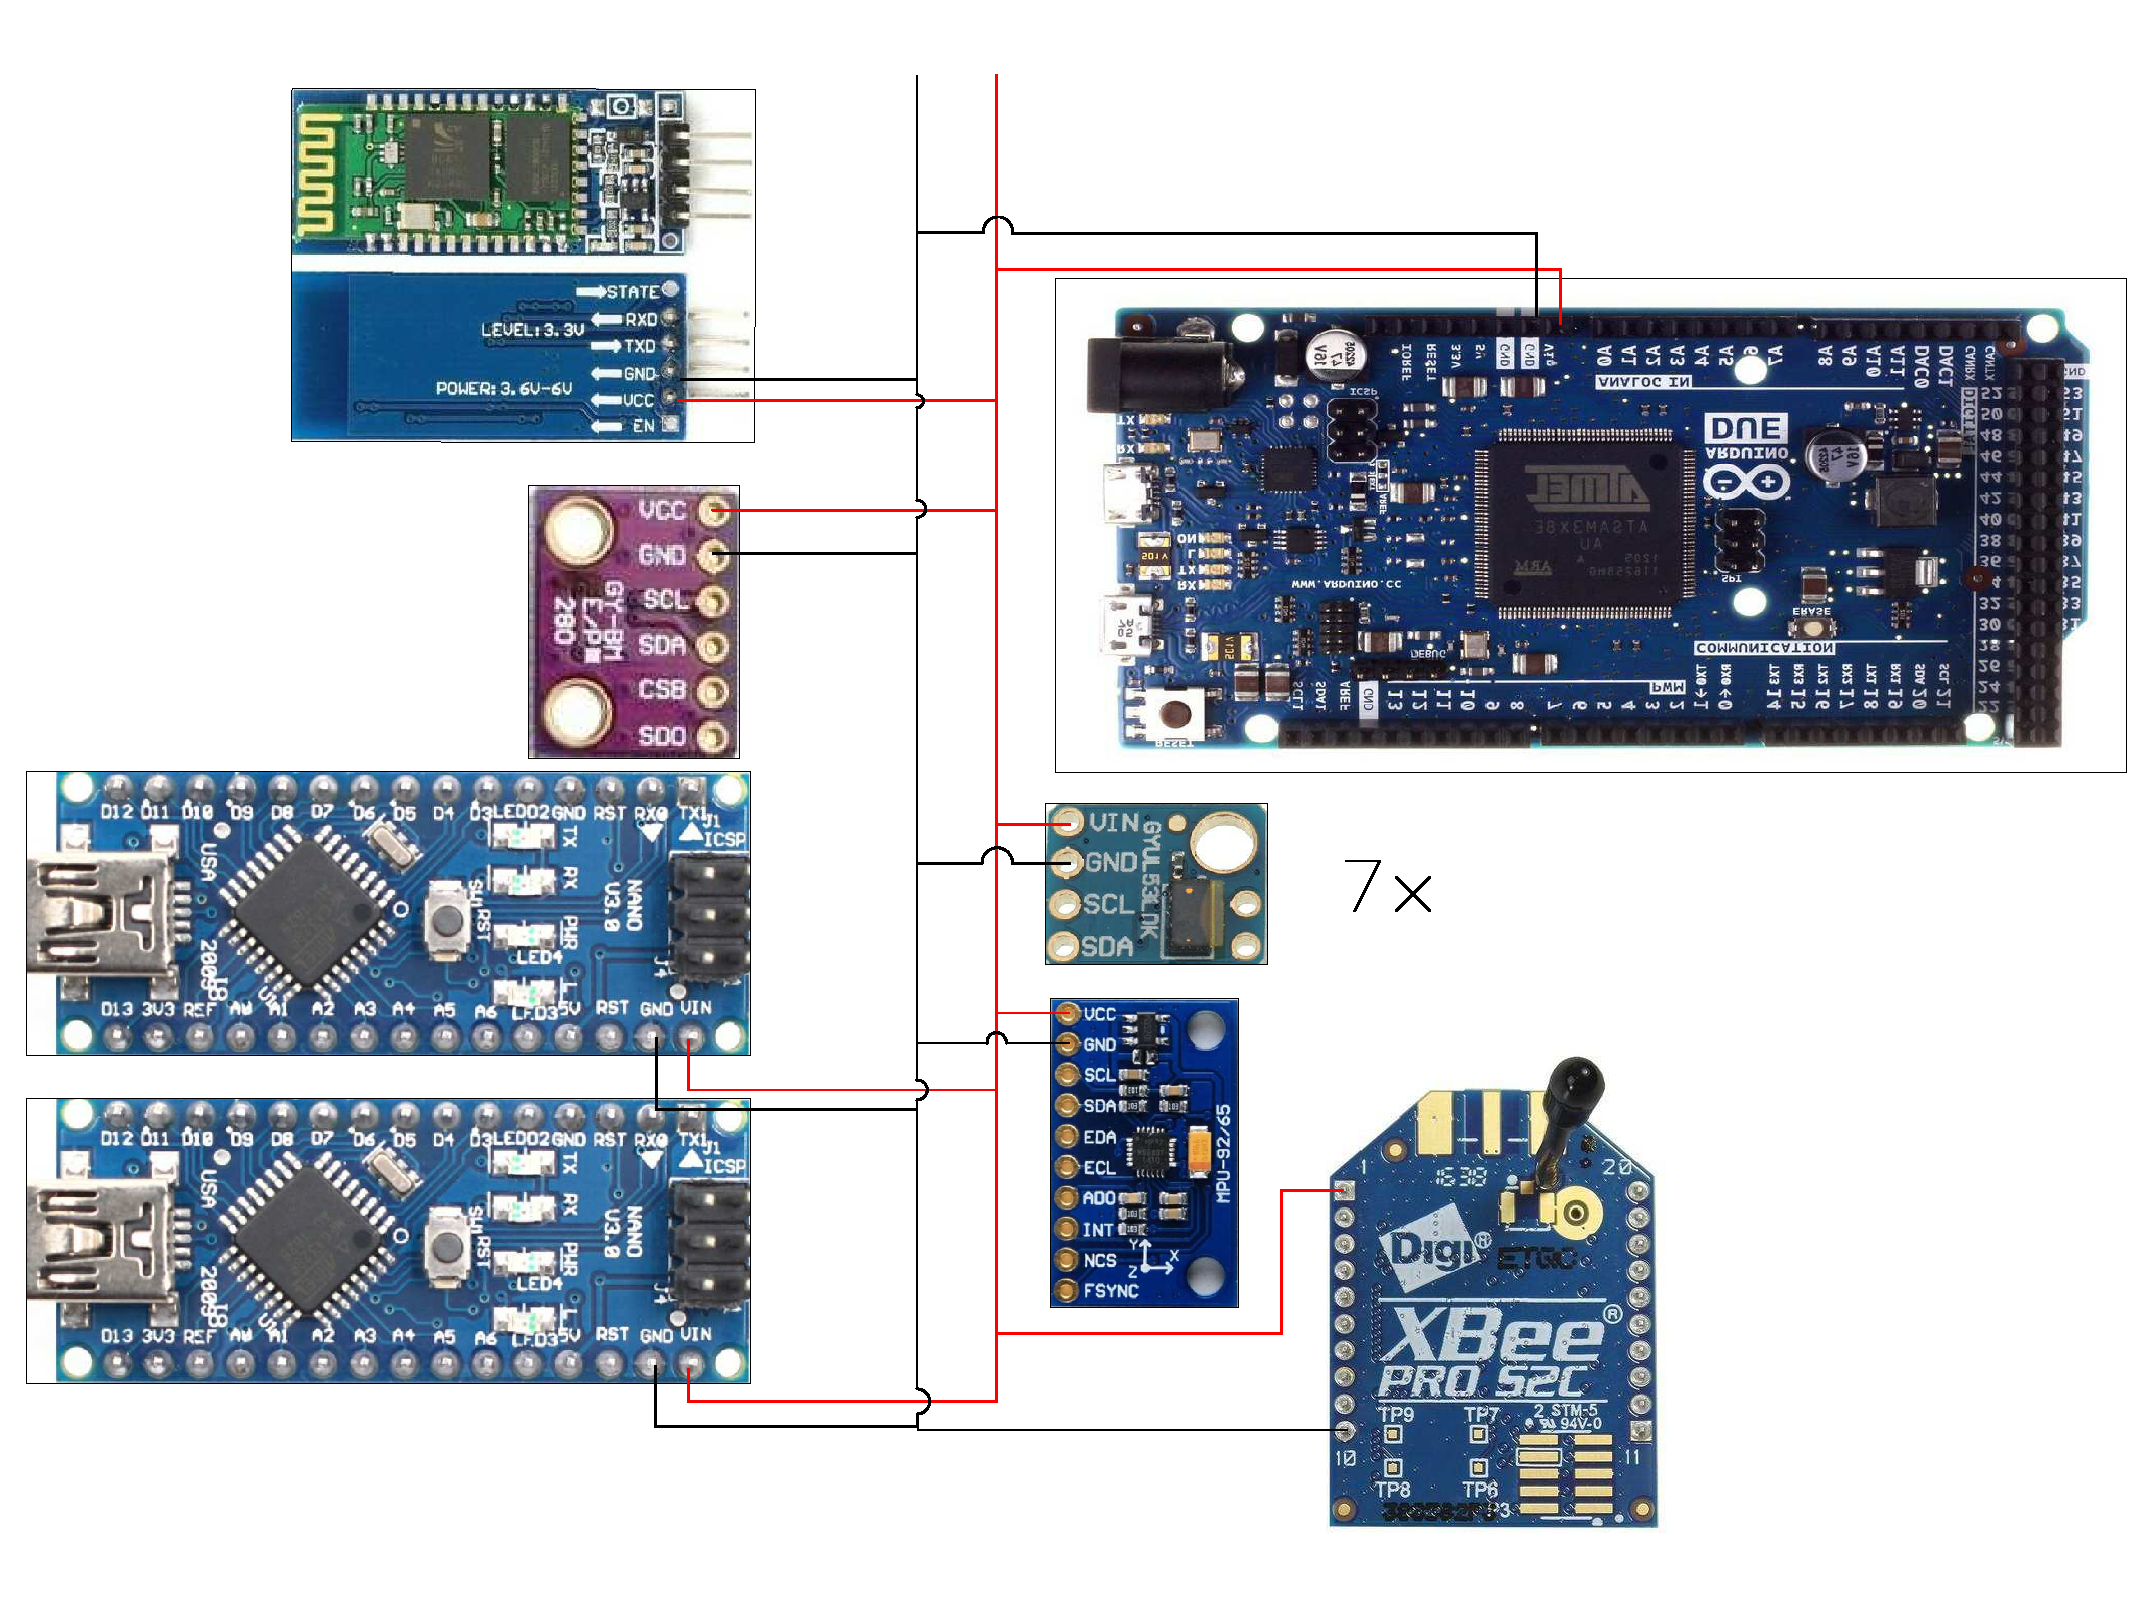
\includegraphics[width=10cm]{pictures/pdb_ardu.pdf}
	\caption{Schéma zapojení napájení Arduina a modulů}
\end{figure}
\begin{figure}[H]
	\centering
	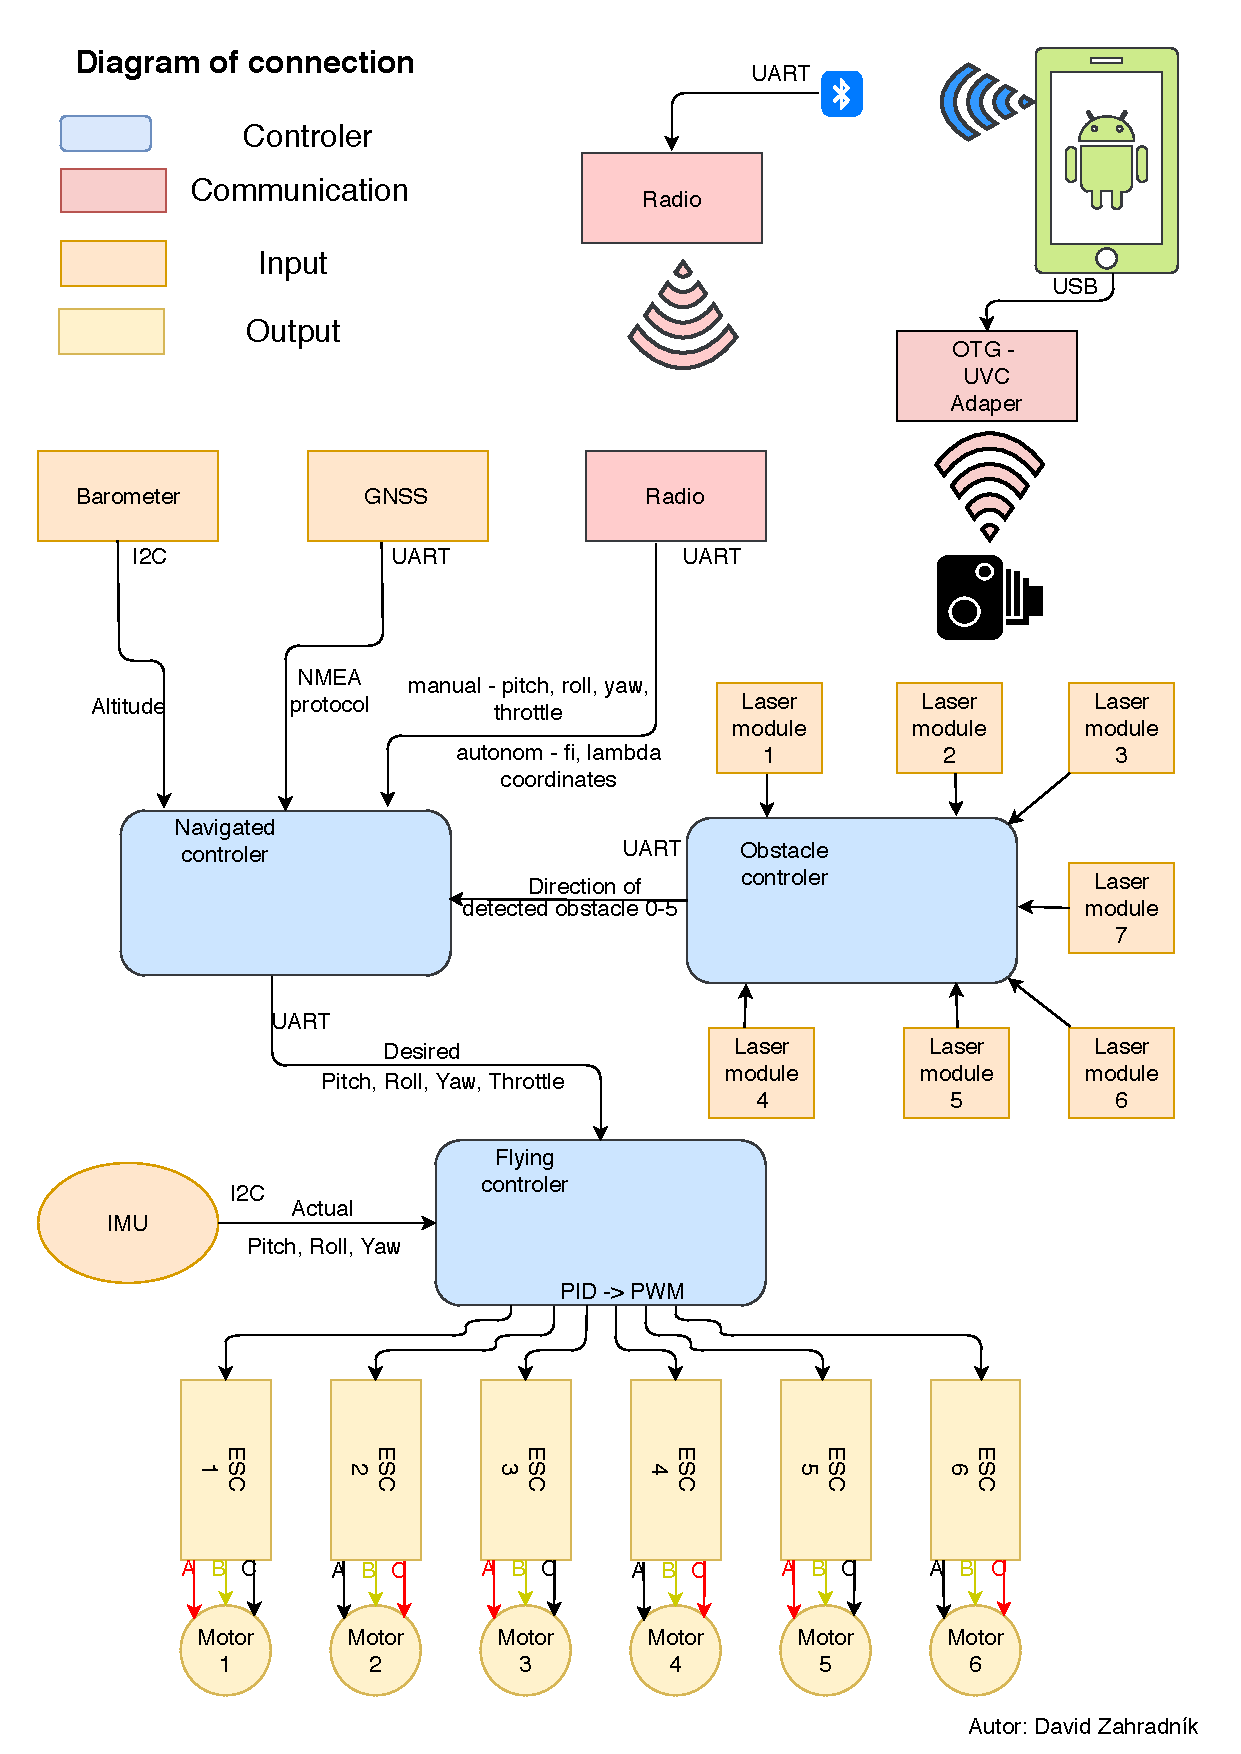
\includegraphics[width=15cm]{pictures/DroneDiagram.pdf}
	\caption{Diagram komponent}
\end{figure}
\begin{figure}[h]
	\centering
	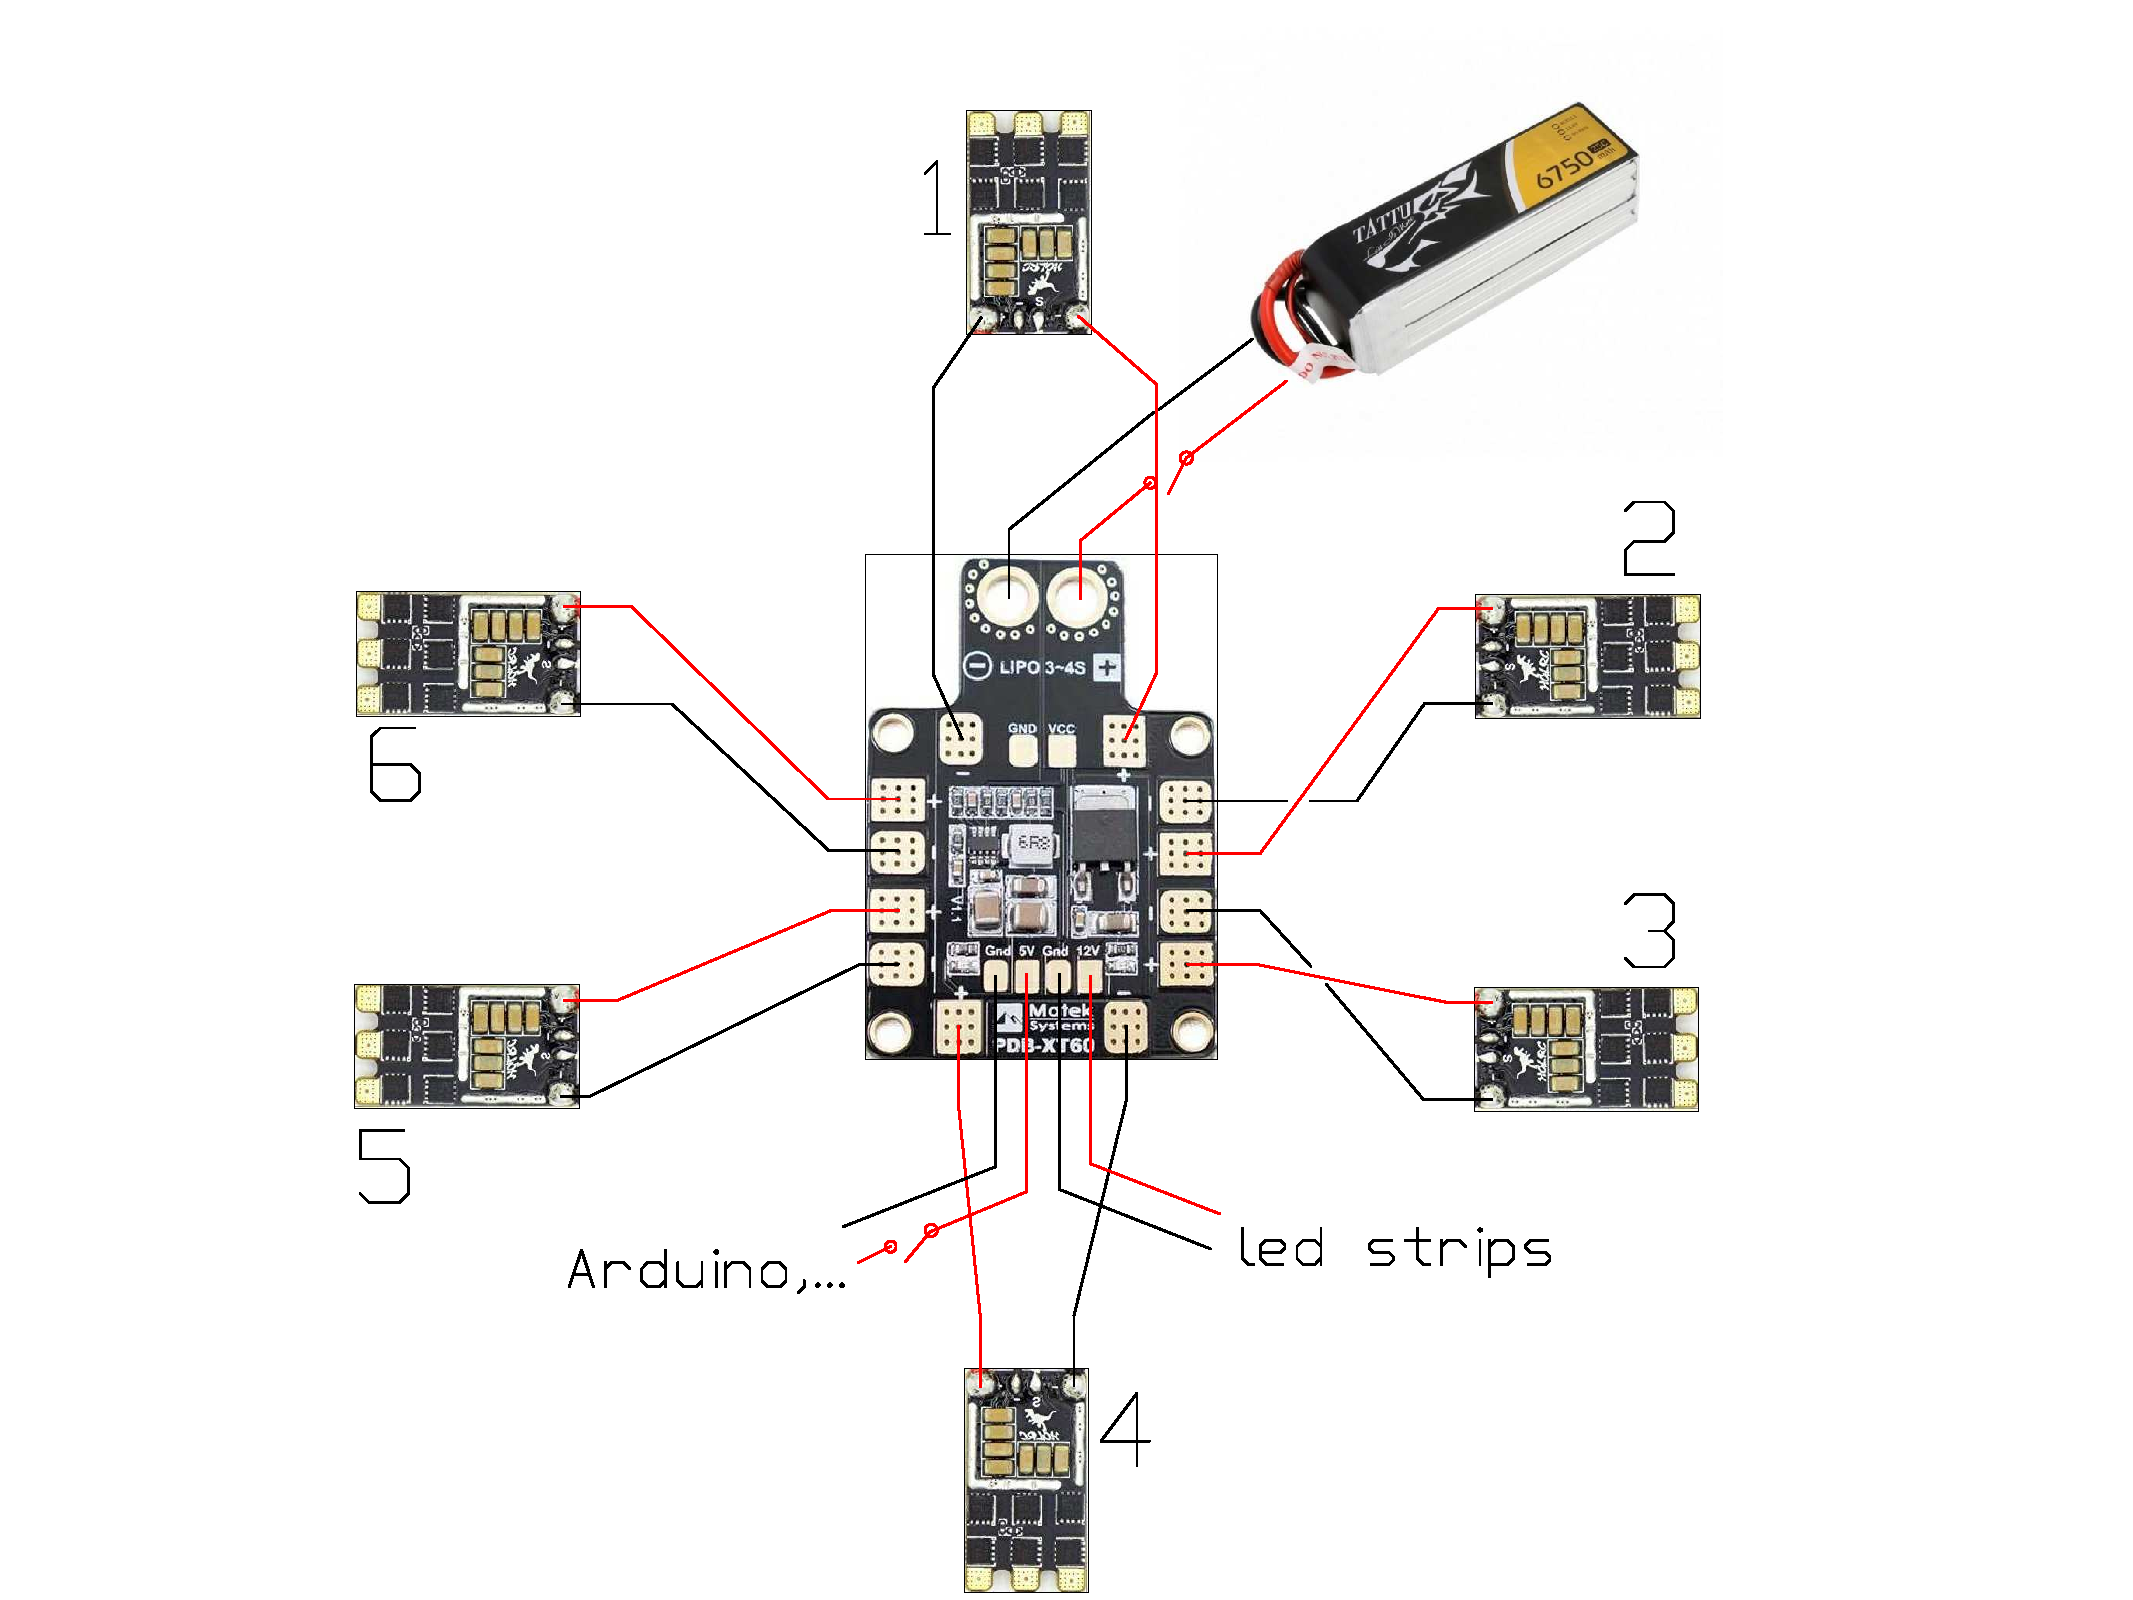
\includegraphics[width=10cm]{pictures/pdb_com.pdf}
	\caption{Schéma zapojení napájení motorů}
\end{figure}